%% Template for a preprint Letter or Article for submission
%% to the journal Nature.
%% Written by Peter Czoschke, 26 February 2004
%%

\documentclass[12pt]{article}

%% make sure you have the nature.cls and naturemag.bst files where
%% LaTeX can find them

\usepackage{scicite,graphicx,rotating}
\usepackage{times}


\title{Supplementary Material: 
``Climate change decouples drought from early wine grape harvests in Western Europe''}

%% Notice placement of commas and superscripts and use of &
%% in the author list

\author{Benjamin I Cook$^{1,2}$ \& Elizabeth M Wolkovich$^{3,4}$}


\begin{document}

\maketitle

%\subsection*{Model Projections}
%The 21\textsuperscript{st}-century drought projections used output from 17 GCMs in phase 5 of the Coupled Model Intercomparison Project\cite{Taylor2012} (Supplemental Table 1). All models represent one or more continuous ensemble members from the historical (1850--2005 CE) and RCP 8.5 (2006--2099 CE) emission scenarios. We used the same methodology as Ref. 2 to calculate model PDSI for the full interval (1850--2099 CE), using the Penman-Monteith formulation of potential evapotranspiration. The baseline period for calibrating and standardizing the model PDSI anomalies was 1931--1990 CE, the same baseline period as the NADA PDSI. Negative model PDSI values therefore indicate drier conditions than the 1931-1990 period.\\


%% TABLE: MEAN DATES
\begin{sidewaystable}
%\begin{table}
\small
\caption{\small Regional GHD series from DAUX used in construction of the GHD-Core composite series. Included are the codes for each site, their geographic locations (units of decimal degrees), and their mean harvest dates for various intervals.}
\centering
\begin{tabular}{| l l | r r | c c c c c p{5cm} |}
\hline
 \bf GHD Series & \bf Site Code & \bf Lat & \bf Lon & \bf 1600-1900 & \bf 1600-1980 & \bf 1901-1950 & \bf 1951-1980 & \bf 1981-2007 \\
\hline
Alsace	& Als & 48.17 & 7.28 & 282.81 & 281.87 & 272.12 & 287.16	 & 277.70 \\
Bordeaux	& Bor	& 45.18 & -0.75	& 269.01 & 	268.22	&  263.85 &  270.41 &  259.75\\
Burgundy	& Bur	& 47.32	& 5.04	& 269.92	& 270.07	& 269.44	& 272.58	& 262.15\\
Champagne 1	& Cha1	& 47.98	& 4.28	& 266.88	& 267.52	& 267.01	& 270.02	& 264.92\\
Low Loire Valley	& LLV	& 47.15	& 0.22	& 286.12	& 284.61	& 282.69	& 282.56	& 275.33\\
Southern Rhone Valley	& SRv	& 43.98	& 5.05	& 269.20	& 269.10	& 268.84	& 268.46	& 257.87\\
Switzerland (Lake Geneva)	& Swi	& 46.57	& 6.52	& 286.39	& 283.87	& 273.86	& 275.22	& 263.00\\
\hline
\end{tabular}
\end{sidewaystable}

%% TABLE: SERIAL COMPLETION
%\begin{sidewaystable}
\begin{table}
\small
\caption{\small For various intervals , the fraction of years for each regional GHD series for which observations are available.}
\centering
\begin{tabular}{l c c c c c}
\hline
 & \bf 1354-2007 & \bf 1600-1900 & \bf 1600-2007 & \bf 1800-2007 & \bf 1900-2007\\
\hline
Als	& 0.400612 & 0.578073 & 0.642157 & 0.836538	 & 0.824074\\
Bor	 & 0.500000 & 0.647841 & 0.737745 & 0.995192 & 0.990741\\
Bur & 	0.925076	& 0.996678	& 0.990196	& 0.985577	& 0.972222\\
Cha2	& 0.279817	& 0.259136	& 0.448529	& 0.879808	& 0.981481\\
LLV	& 0.310398	& 0.332226	& 0.497549	& 0.975962	& 0.962963\\
SRv	& 0.689602	& 0.970100	& 0.950980	& 0.942308	& 0.898148\\
Swi 	& 0.749235	& 1.000000	& 1.000000	& 1.000000	& 1.000000\\
\hline
\end{tabular}
\end{table}
%\end{sidewaystable}

%% TABLE: CROSS SITE CORRELATIONS
%\begin{sidewaystable}
\begin{table}
\small
\caption{\small Spearman's rank correlations (1600-2007) between each regional GHD series used in construction of the GHD-Core index.}
\centering
\begin{tabular}{c c c c c c c c}
\hline
& Als & Bor & Bur & Cha1 & LLV & SRv & Swi \\
\hline
Als	& 1	& 0.601045	& 0.573844	& 0.632206	& 0.502502	& 0.413751	& 0.604378\\
Bor & 0.601045 	& 1	& 0.622279		& 0.675208	& 0.712442 	& 0.321238 	& 0.547885\\
Bur &	0.573844	& 0.622279	& 1	& 0.798581	& 0.775801	& 0.542594	& 0.582605\\
Cha1	& 0.632206	& 0.675208	& 0.798581	& 1	 & 0.709044	& 0.346222	& 0.569444\\
LLV	& 0.502502	& 0.712442	& 0.775801	& 0.709044	& 1 & 0.456008 & 0.696642\\
SRv	& 0.413751	& 0.321238	& 0.542594	& 0.346222	& 0.456008	& 1	 & 0.525608\\
Swi	 & 0.604378	& 0.547885	& 0.582605	& 0.569444	& 0.696642	& 0.525608	& 1\\
\hline
\end{tabular}
%\end{sidewaystable}
\end{table}

%% TABLE: GHD ANOMALIES
%\begin{sidewaystable}
\begin{table}
\small
\caption{\small Anomalies in GHD, calculated relative to the baseline mean baseline calculated for 1600-1900. Also included are results for the GHD-Core index and GHD-All, composited from all 27 regional GHD series in DAUX. GHD-Core and GHD-All represent the composite average AFTER the anomalysing of the individual regional GHD series.}
\centering
\begin{tabular}{l c c c c c}
\hline
& \bf 1600-1900 & \bf 1600-1980 & \bf 1901-1950 & \bf 1951-1980 & \bf 1981-2007\\
\hline
Als	& 0	& -0.94 & -10.69 & 4.35 & -5.11\\
Bor	& 0 & -0.79 & -5.16 & 1.40 & -9.26\\
Bur	& 0	& 0.15	& -0.48	& 2.66	& -7.78\\
Cha1	& 0	& 0.64	& 0.13	& 3.14	& -1.96\\
LLV	& 0	& -1.51	& -3.42	& -3.56	& -10.79\\
SRv & 0	& -0.10	& -0.36	& -0.74	& -11.33\\
Swi	& 0	& -2.52	& 12.53	& 11.17	& 23.39\\
\hline
GHD-Core & -0.35 & -0.91	& -4.49 & -0.47 & 	-10.62\\
GHD-All	& -0.25 & -0.85 & -5.13 & 0.36 & -8.91\\
\hline
\end{tabular}
%\end{sidewaystable}
\end{table}

%% TABLE: GHD STANDARD DEVIATIONS
%\begin{sidewaystable}
\begin{table}
\small
\caption{\small As Table 4, but for inter-annual standard deviation.}
\centering
\begin{tabular}{l c c c c c}
\hline
& \bf 1600-1900 & \bf 1600-1980 & \bf 1901-1950 & \bf 1951-1980 & \bf 1981-2007\\
\hline
Als	& 8.74	& 9.56	& 9.12	& 7.09	& 8.74\\
Bor	& 9.51	& 9.00	& 6.27	& 7.00	& 9.56\\
Bur	& 9.61 & 9.19 & 6.55 & 8.11 & 7.97\\
Cha1 & 8.81 & 8.88 & 7.85 & 10.12 & 8.64\\
LLV	& 10.29 & 9.21 & 6.56 & 8.01 & 7.41\\
SRv & 8.68 & 8.46 & 8.62 & 5.55 & 5.93\\
Swi	& 10.09	& 10.71	& 7.19	& 6.68	& 8.11\\
\hline
GHD-Core & 7.80 & 7.57	& 5.50	& 6.61	& 7.92\\
GHD-All	& 7.03 & 7.02 & 5.55 & 6.55 & 6.75\\
\hline
\end{tabular}
%\end{sidewaystable}
\end{table}


\pagebreak

%% THESE COMMANDS ARE USED TO RESET THE SUPPLEMENTAL FIGURE NAMES
\renewcommand{\figurename}{Supplementary Figure}
\setcounter{figure}{0}
%\renewcommand{\thefigure}{}

\begin{figure}
\center
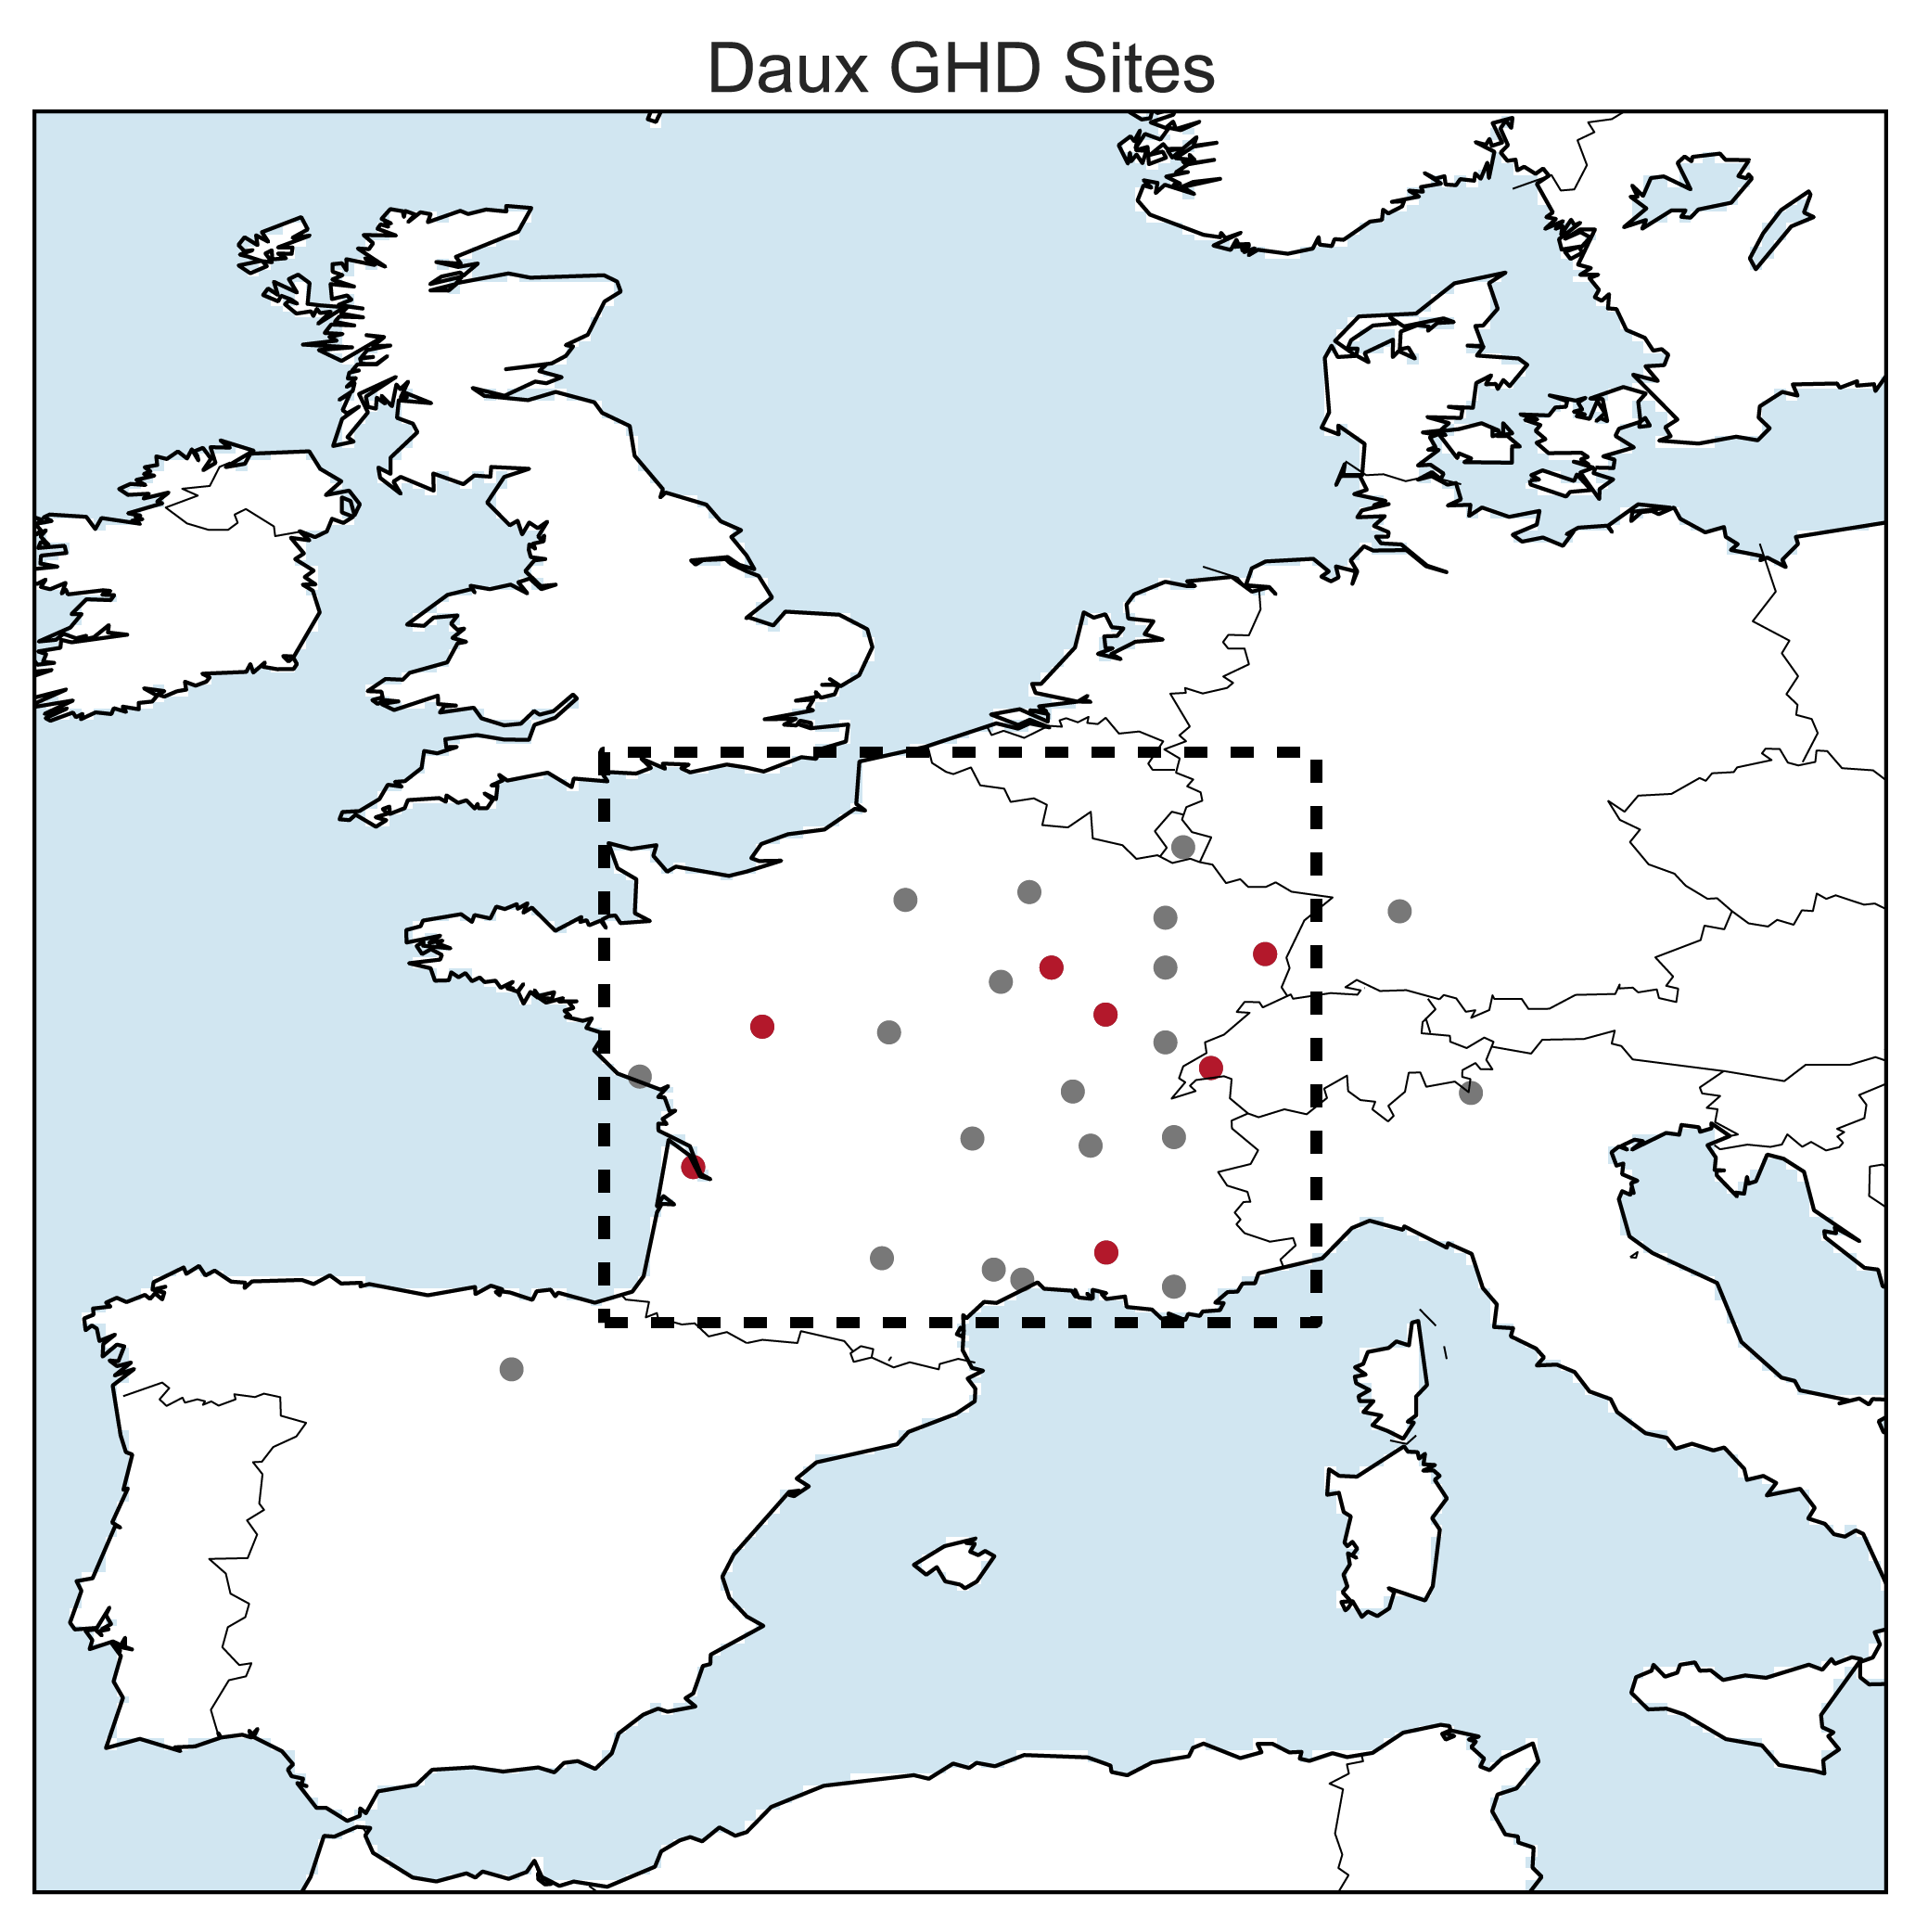
\includegraphics[width=1.0\columnwidth,scale=2]{SUPP_fig_01_map_sitelocs.png}
\caption{Geographic locations for all 27 regional GHD time series in DAUX. Highlighted in red are the sites that comprise the GHD-Core index: Alsace (Als), Bordeaux (Bor), Burgundy (Bur), Champagne 1 (Cha1), the Lower Loire Valley (LLV), the Southern Rhone Valley (SRv), and Switzerland at Lake Geneva (Swi).}
\end{figure}

\begin{figure}
\center
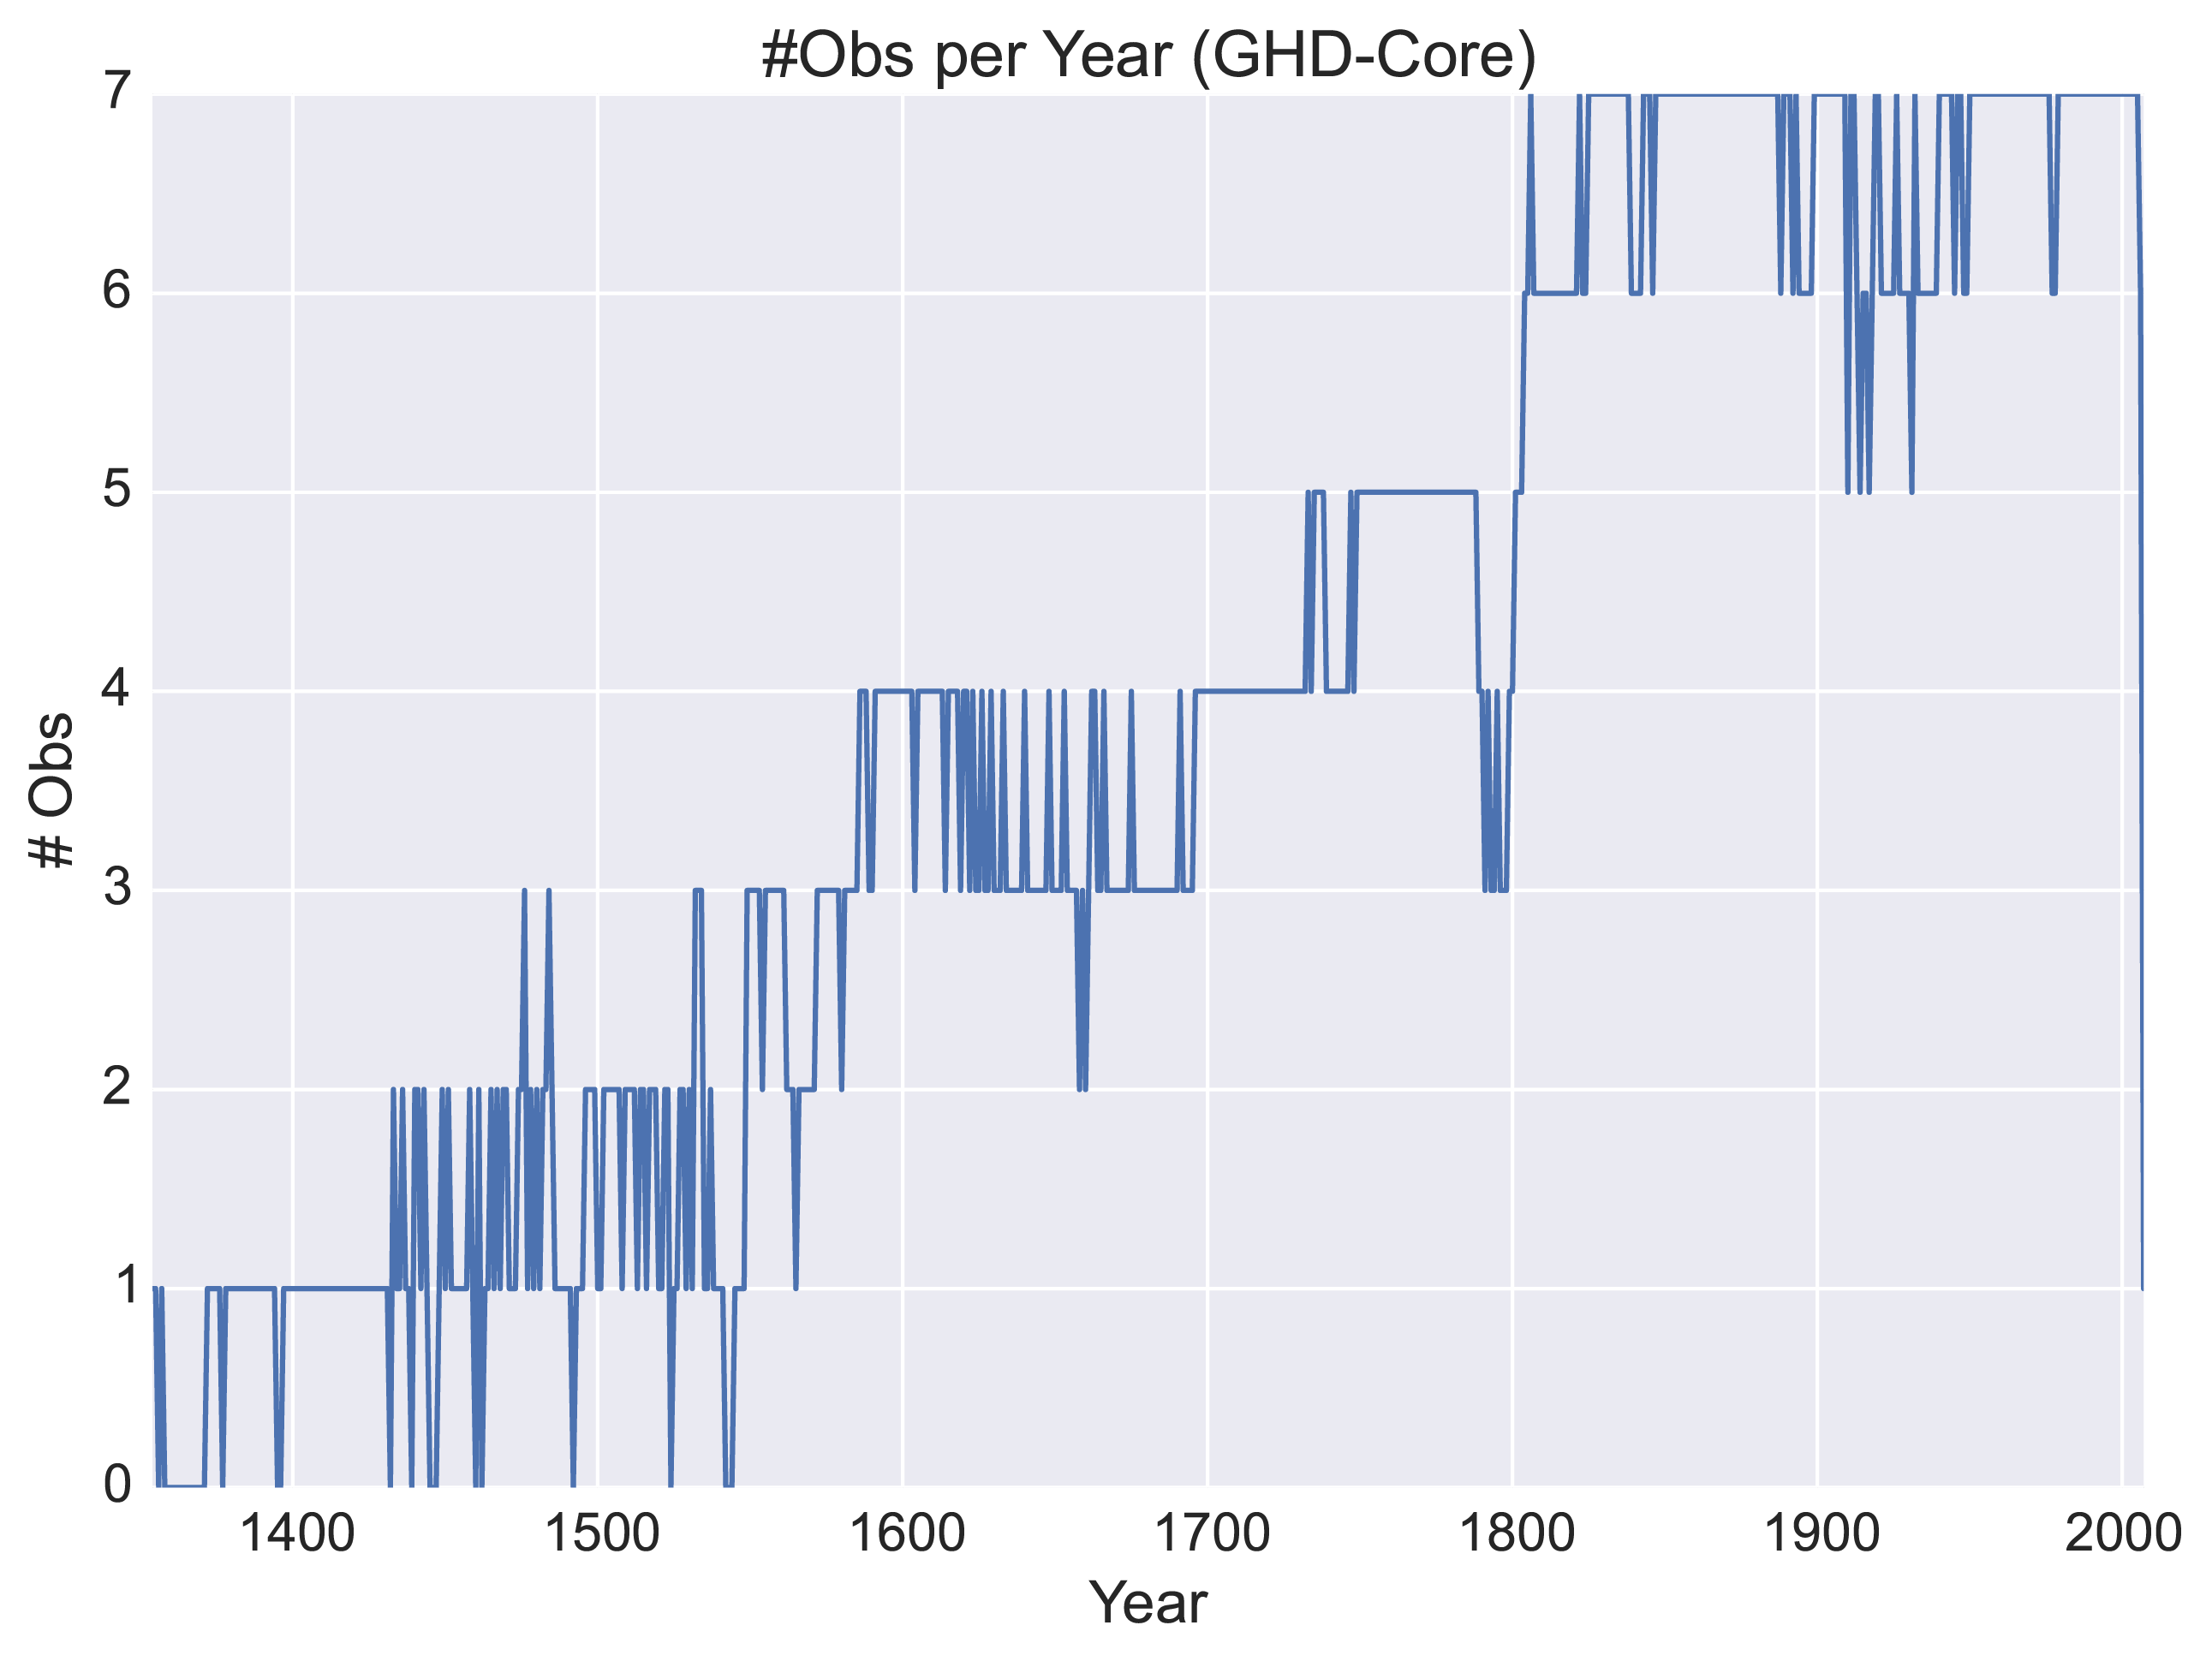
\includegraphics[width=1.0\columnwidth,scale=2]{SUPP_fig_02_numobs.png}
\caption{Number of observations (i.e., regional GHD series) represented in each year of the GHD-Core index.}
\end{figure}

\begin{sidewaysfigure}
\center
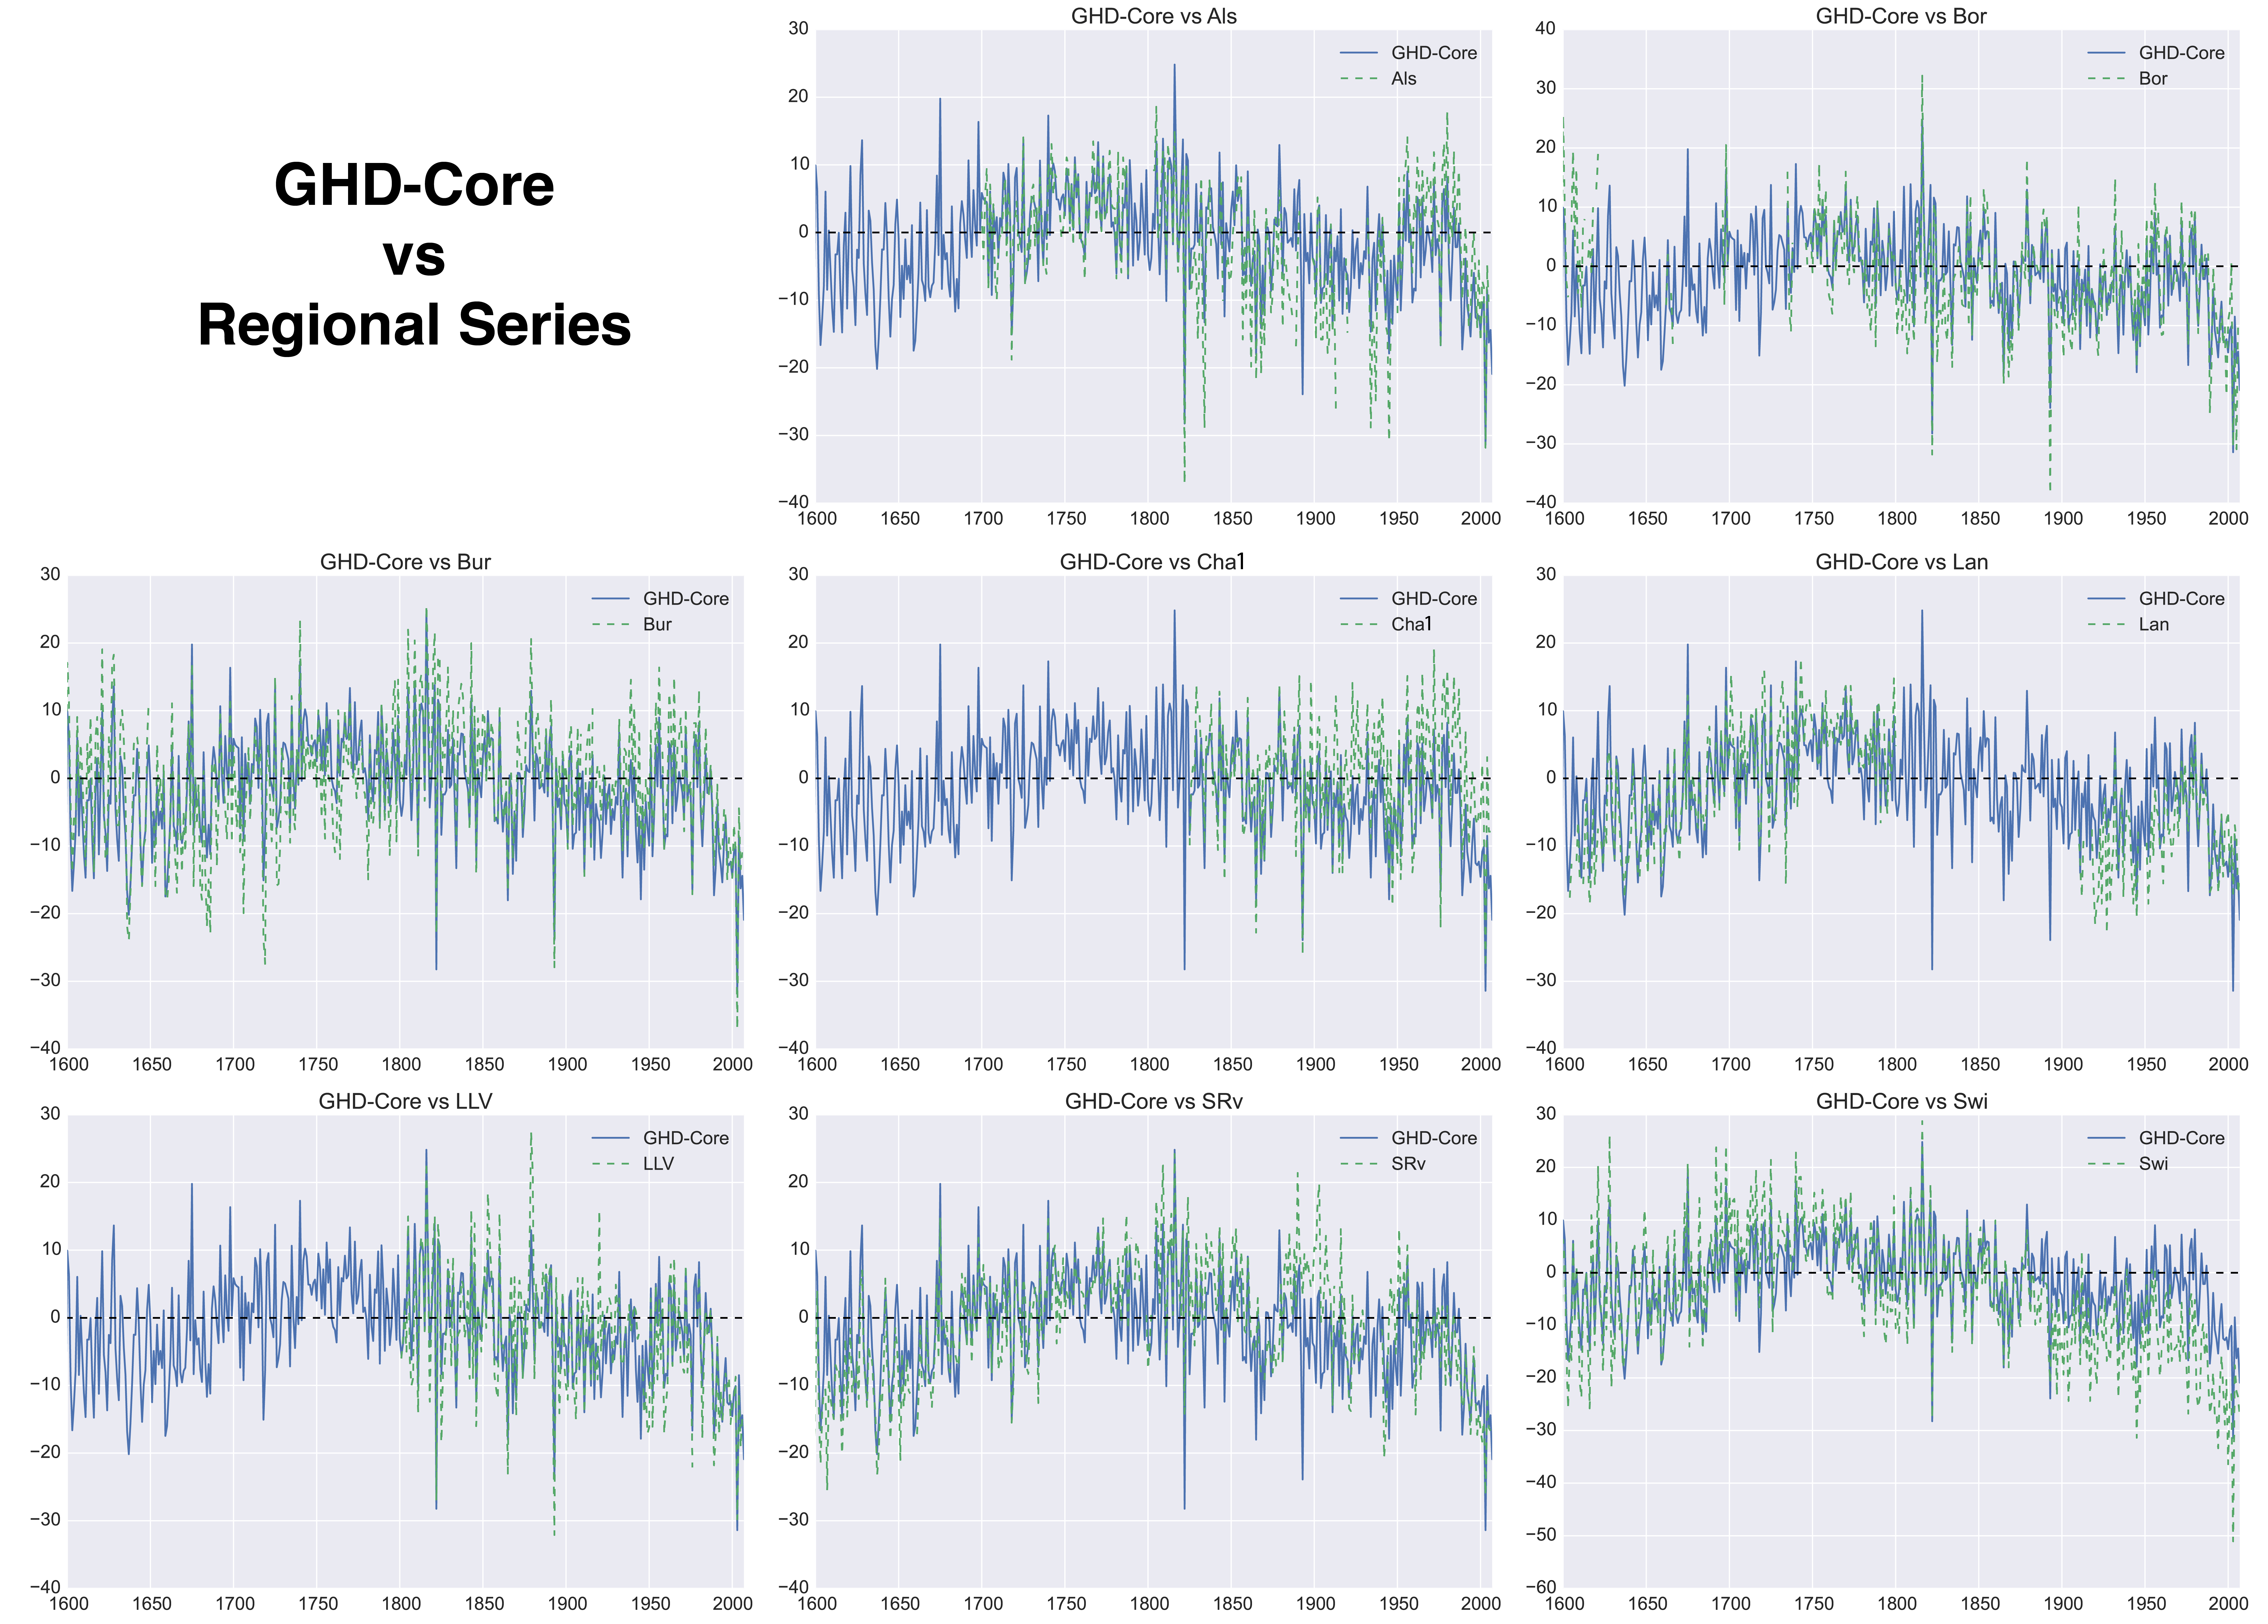
\includegraphics[width=1.0\columnwidth,scale=2]{SUPP_fig_03_core_vs_sites.png}
\caption{Time series (1600--2007) of GHD-Core (blue sold line) and each individual regional GHD series (green dashed lines).}
\end{sidewaysfigure}

\begin{figure}
\center
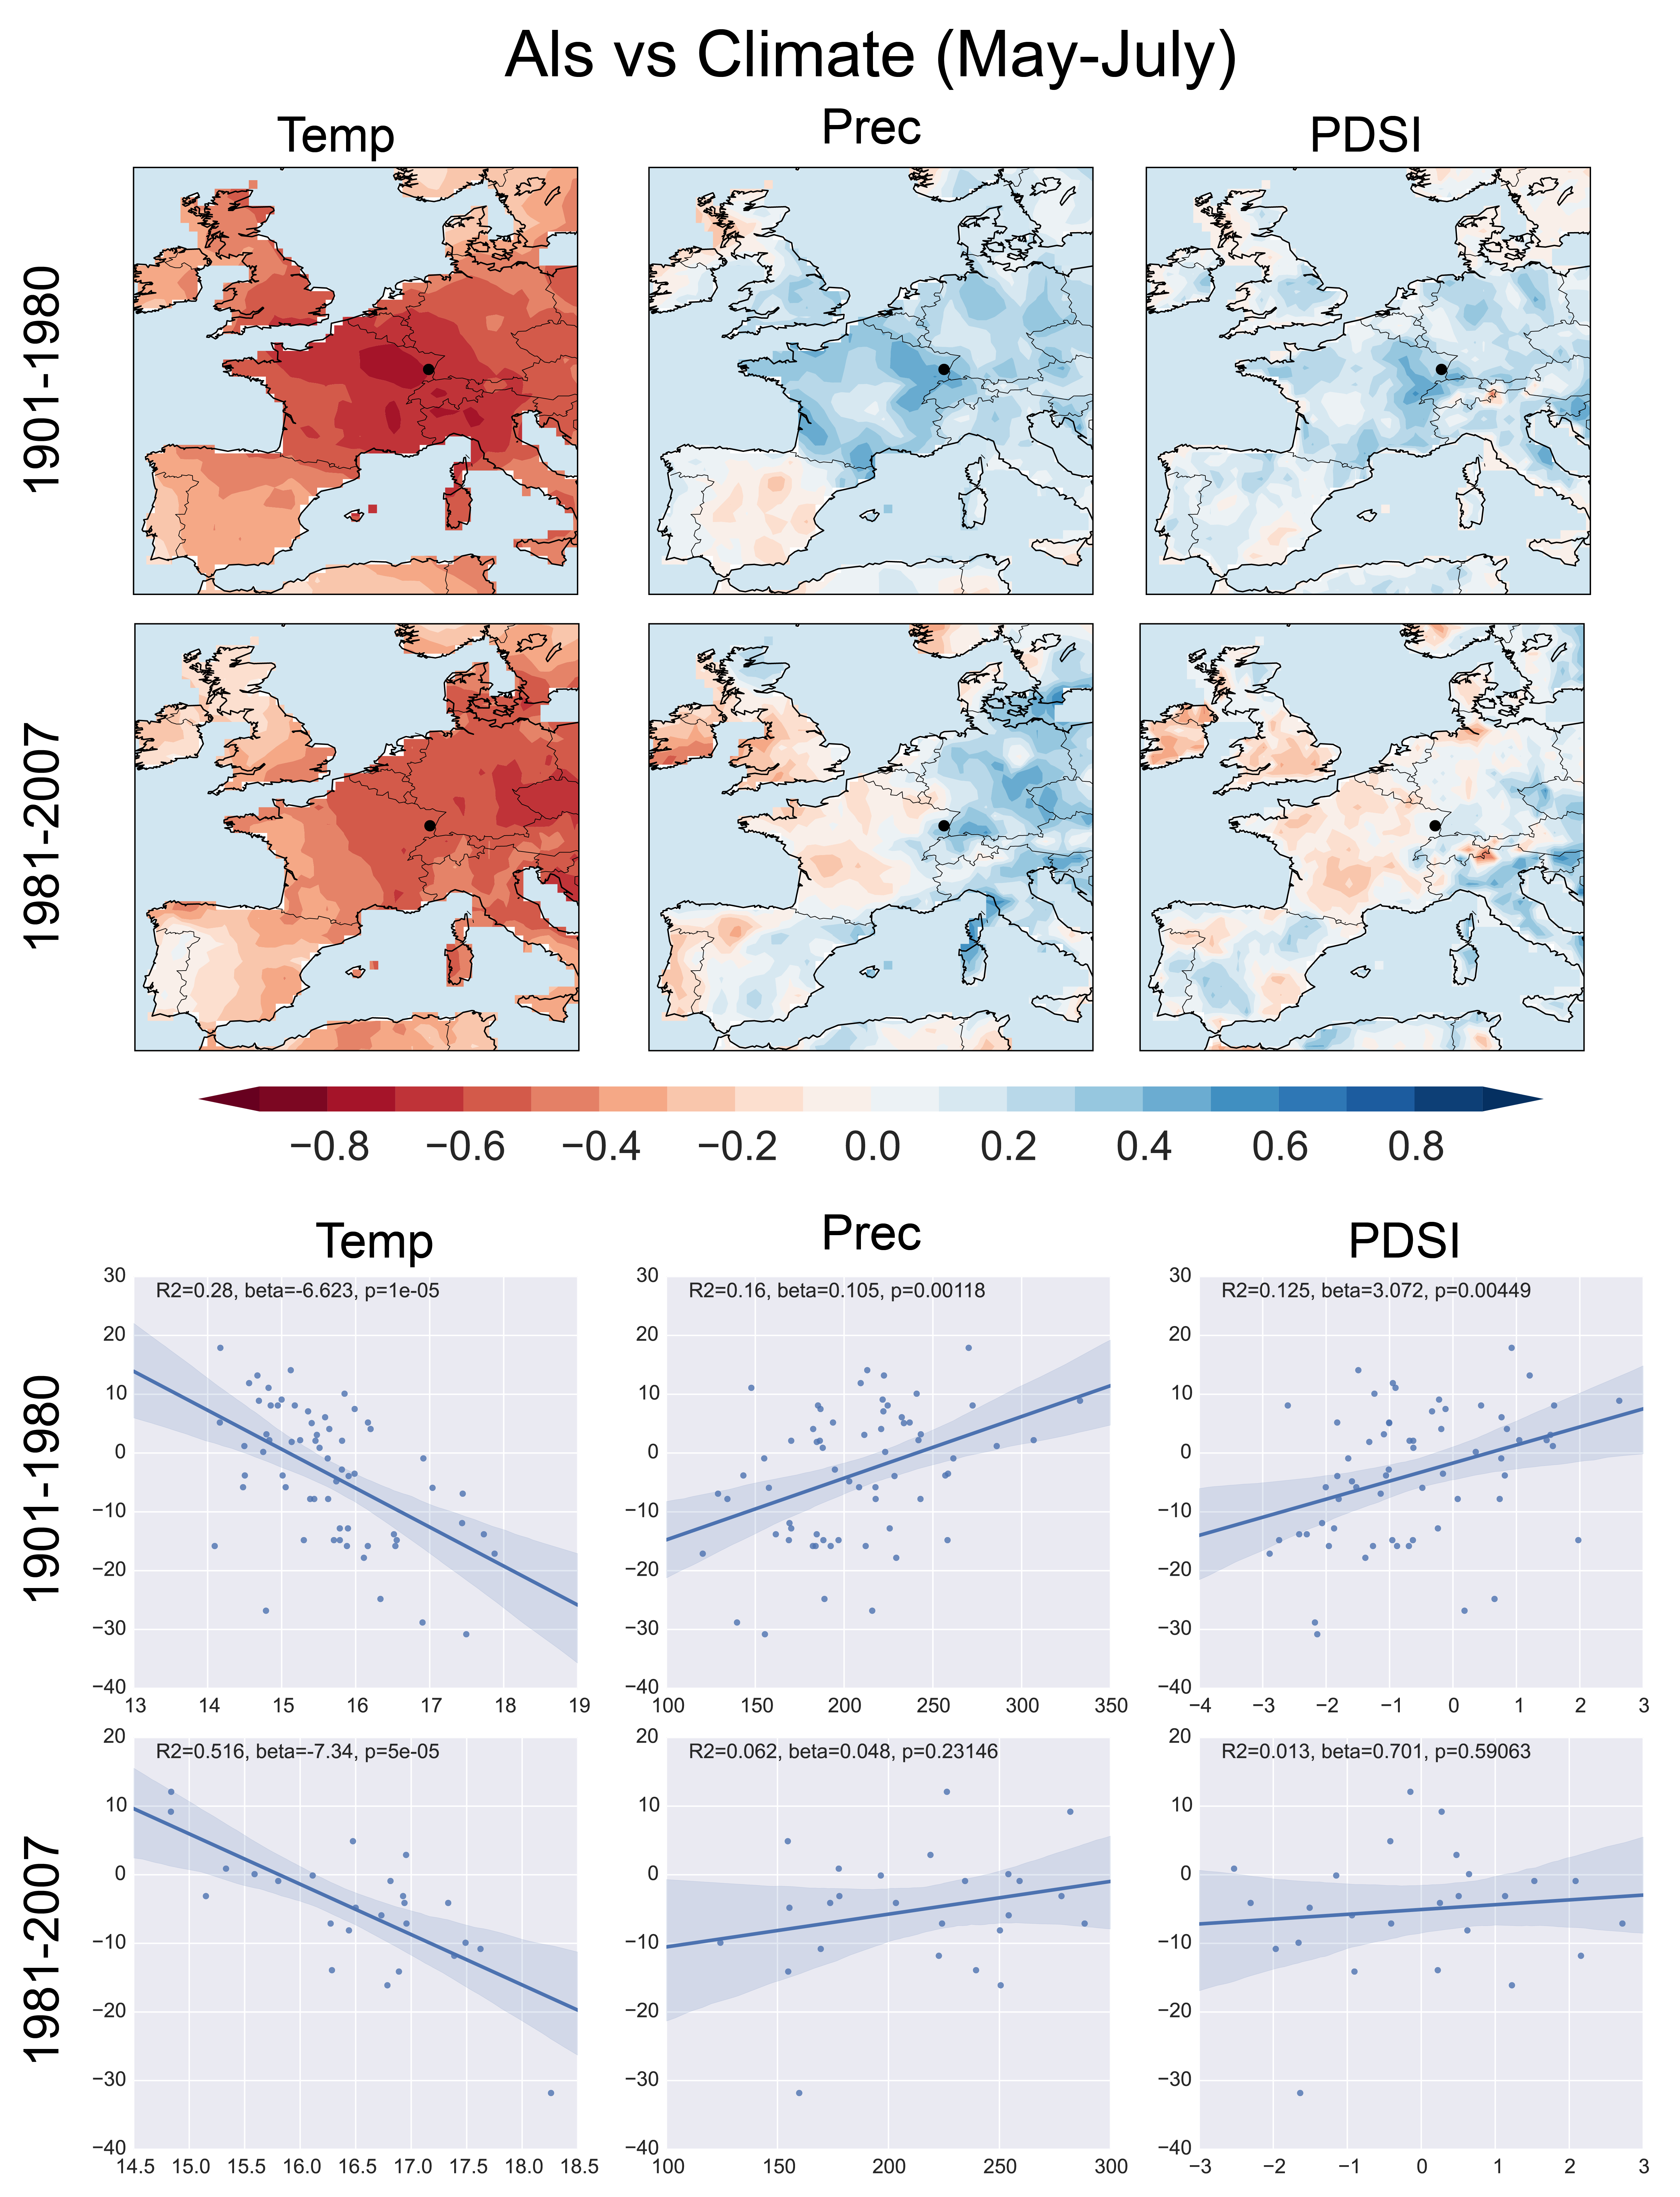
\includegraphics[width=.9\columnwidth,scale=2]{SUPP_fig_04_ALS_MJJ_climate.png}
\caption{Comparisons between the GHD series from ALS and May-June-July temperature, precipitation, and scPDSI from the CRU 3.21 climate grids. Top panels: point-by-point correlations for 1901--1980 and 1981--2007 (location of ALS is shown by the black dot). Bottom panels: linear regression plots for the same intervals against CRU climate data averaged within one degree of the site location.}
\end{figure}

\begin{figure}
\center
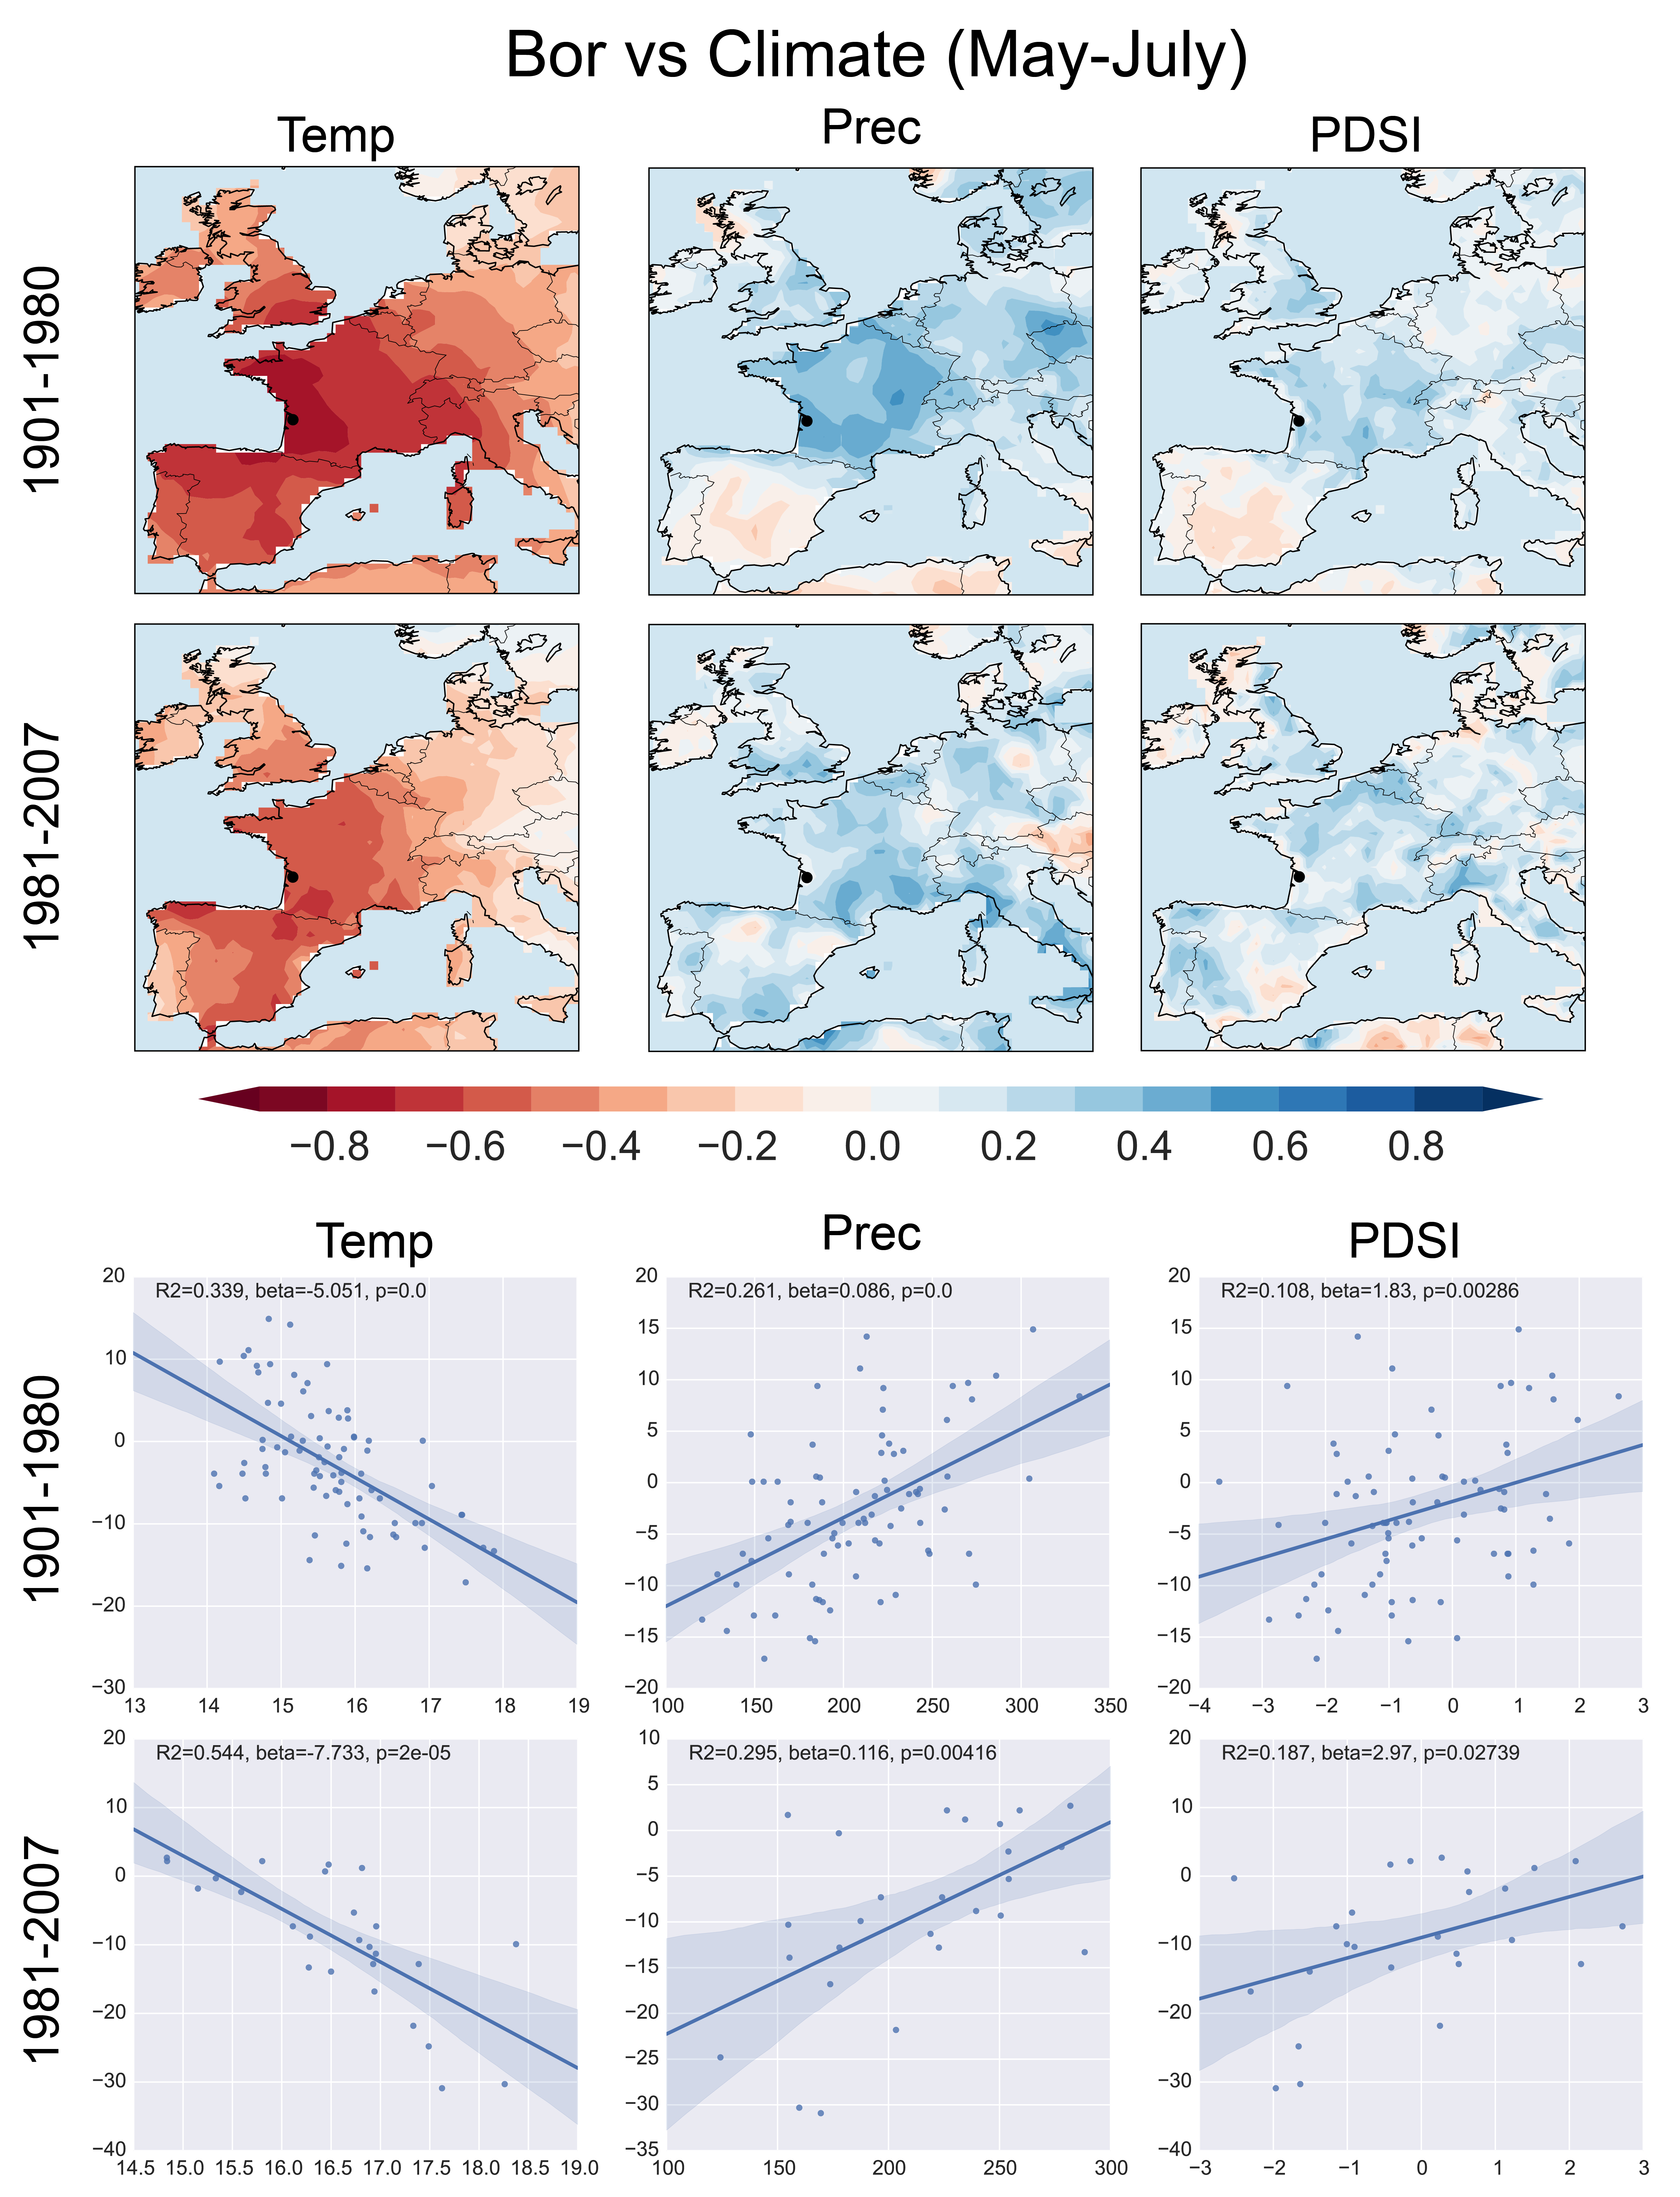
\includegraphics[width=.9\columnwidth,scale=2]{SUPP_fig_05_Bor_MJJ_climate.png}
\caption{Same as Figure 4, but for Bor.}
\end{figure}

\begin{figure}
\center
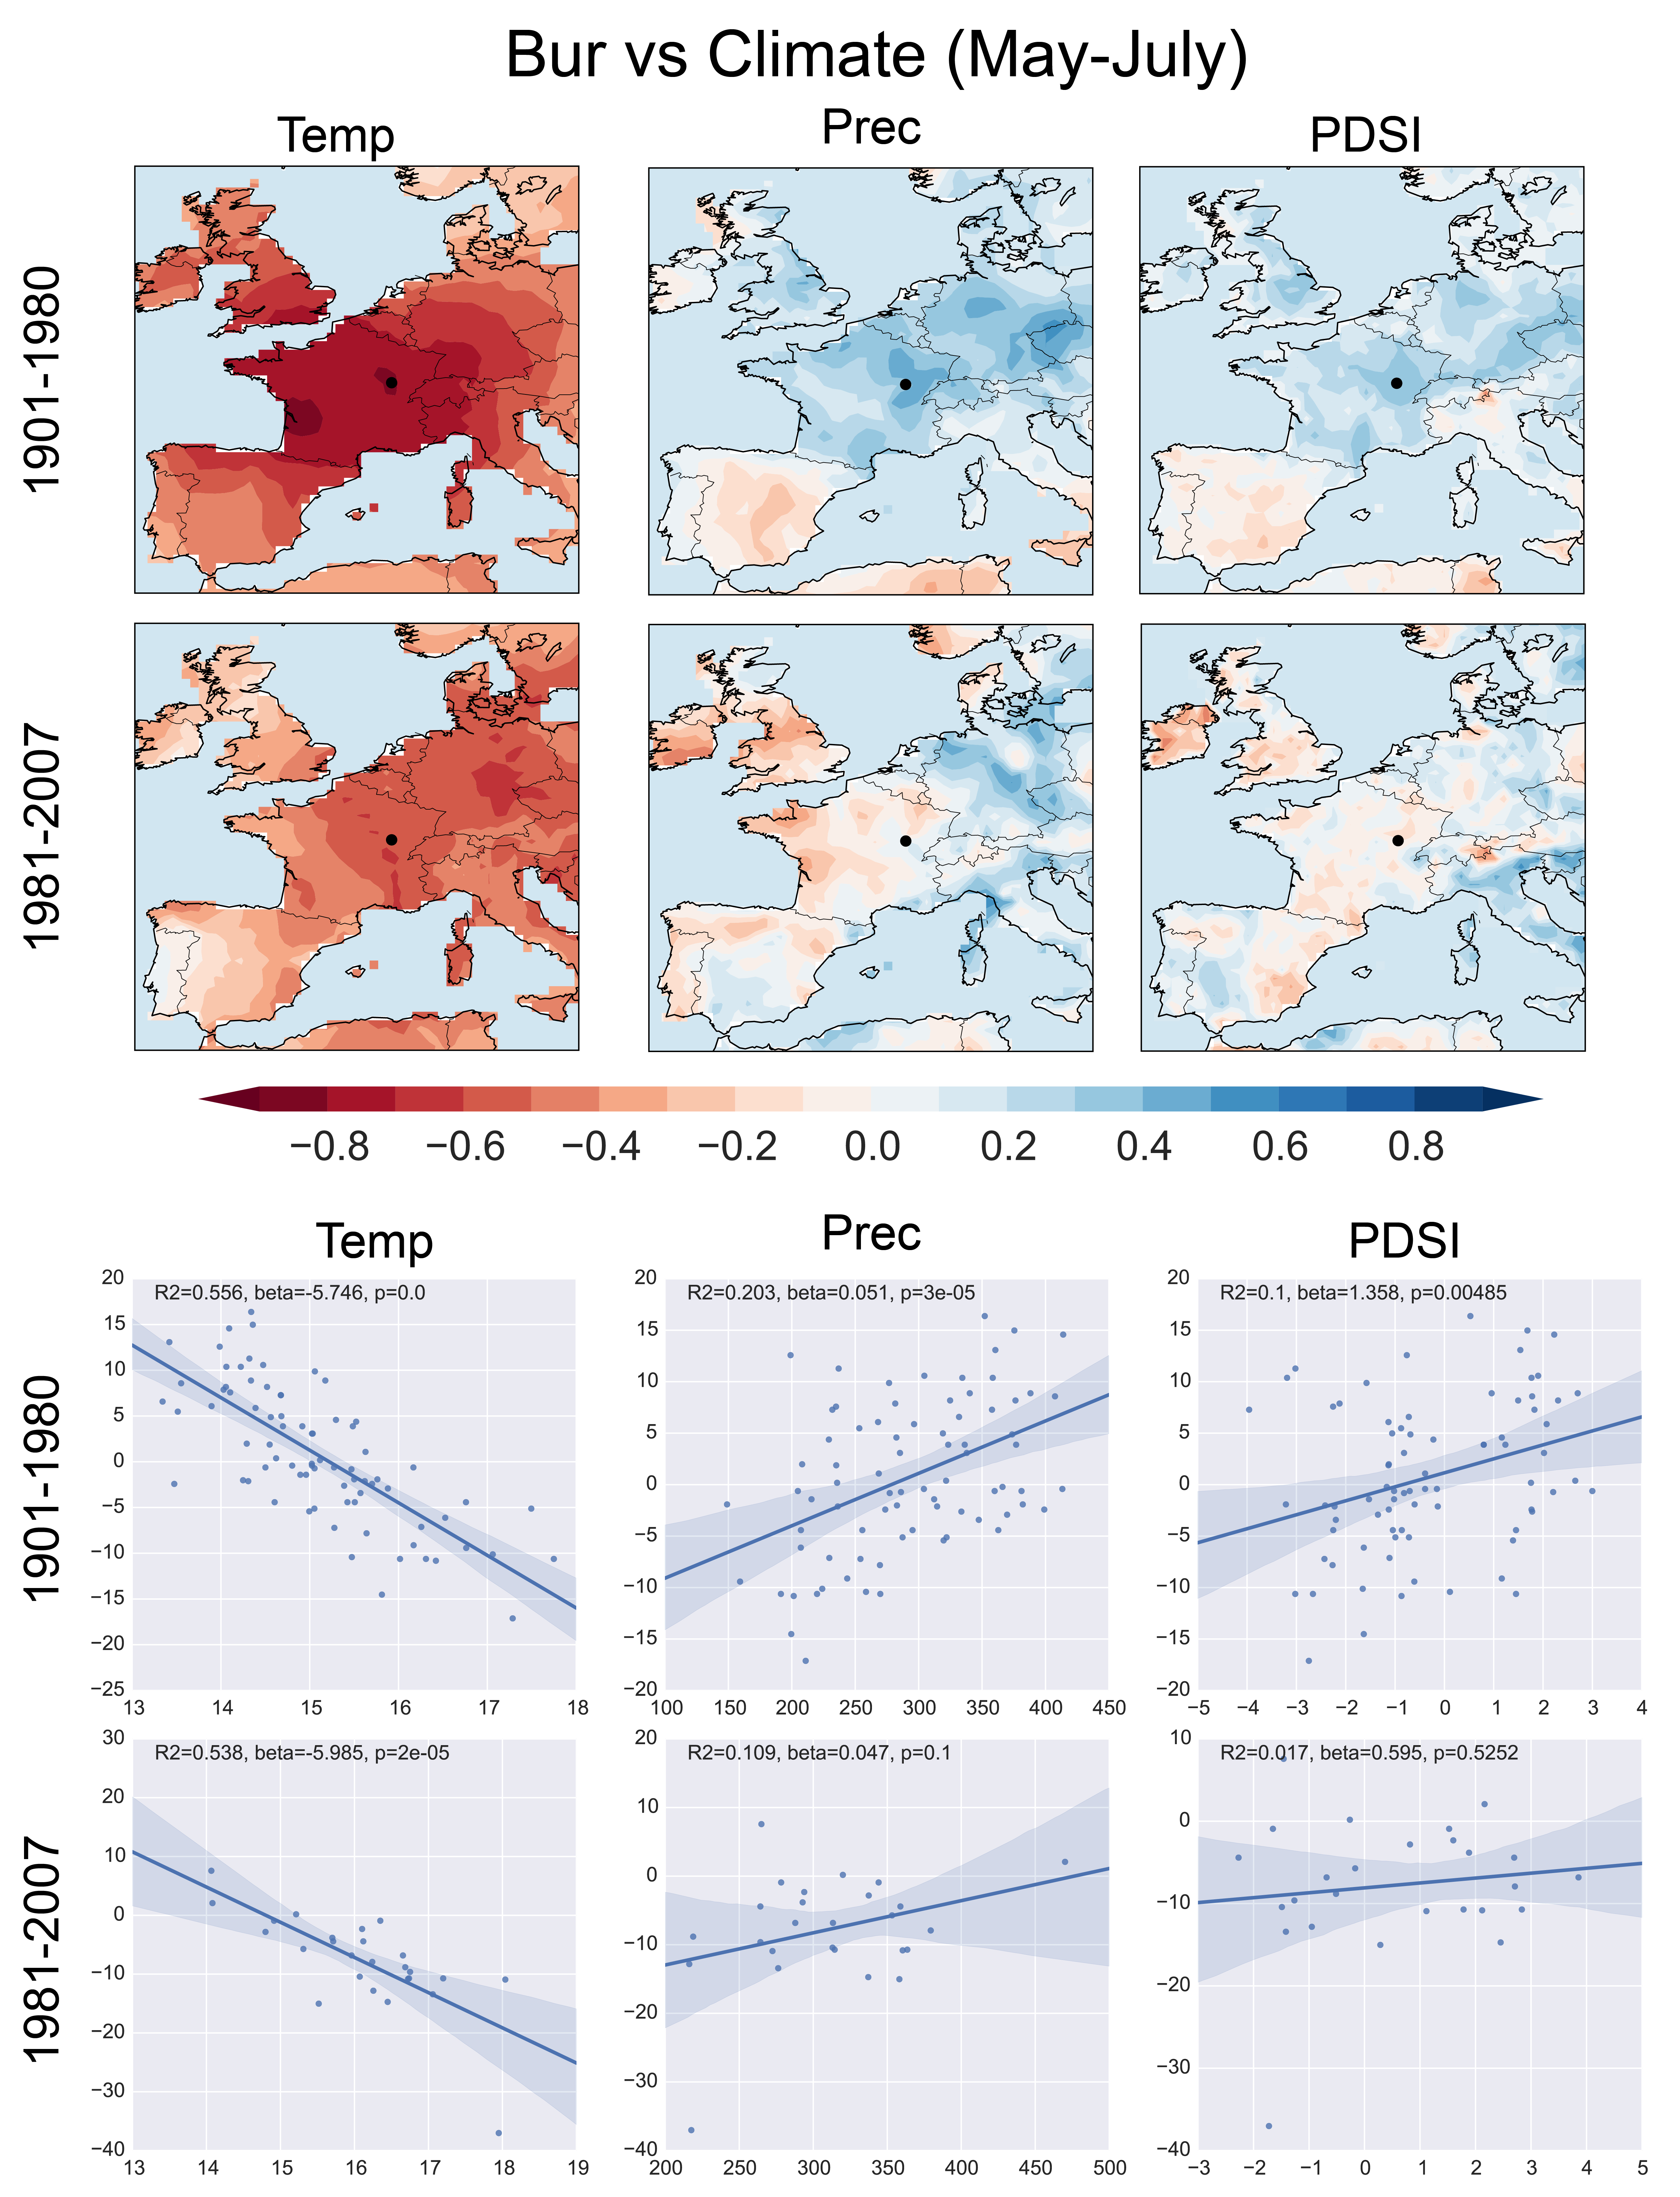
\includegraphics[width=.9\columnwidth,scale=2]{SUPP_fig_06_Bur_MJJ_climate.png}
\caption{Same as Figure 4, but for Bur.}
\end{figure}

\begin{figure}
\center
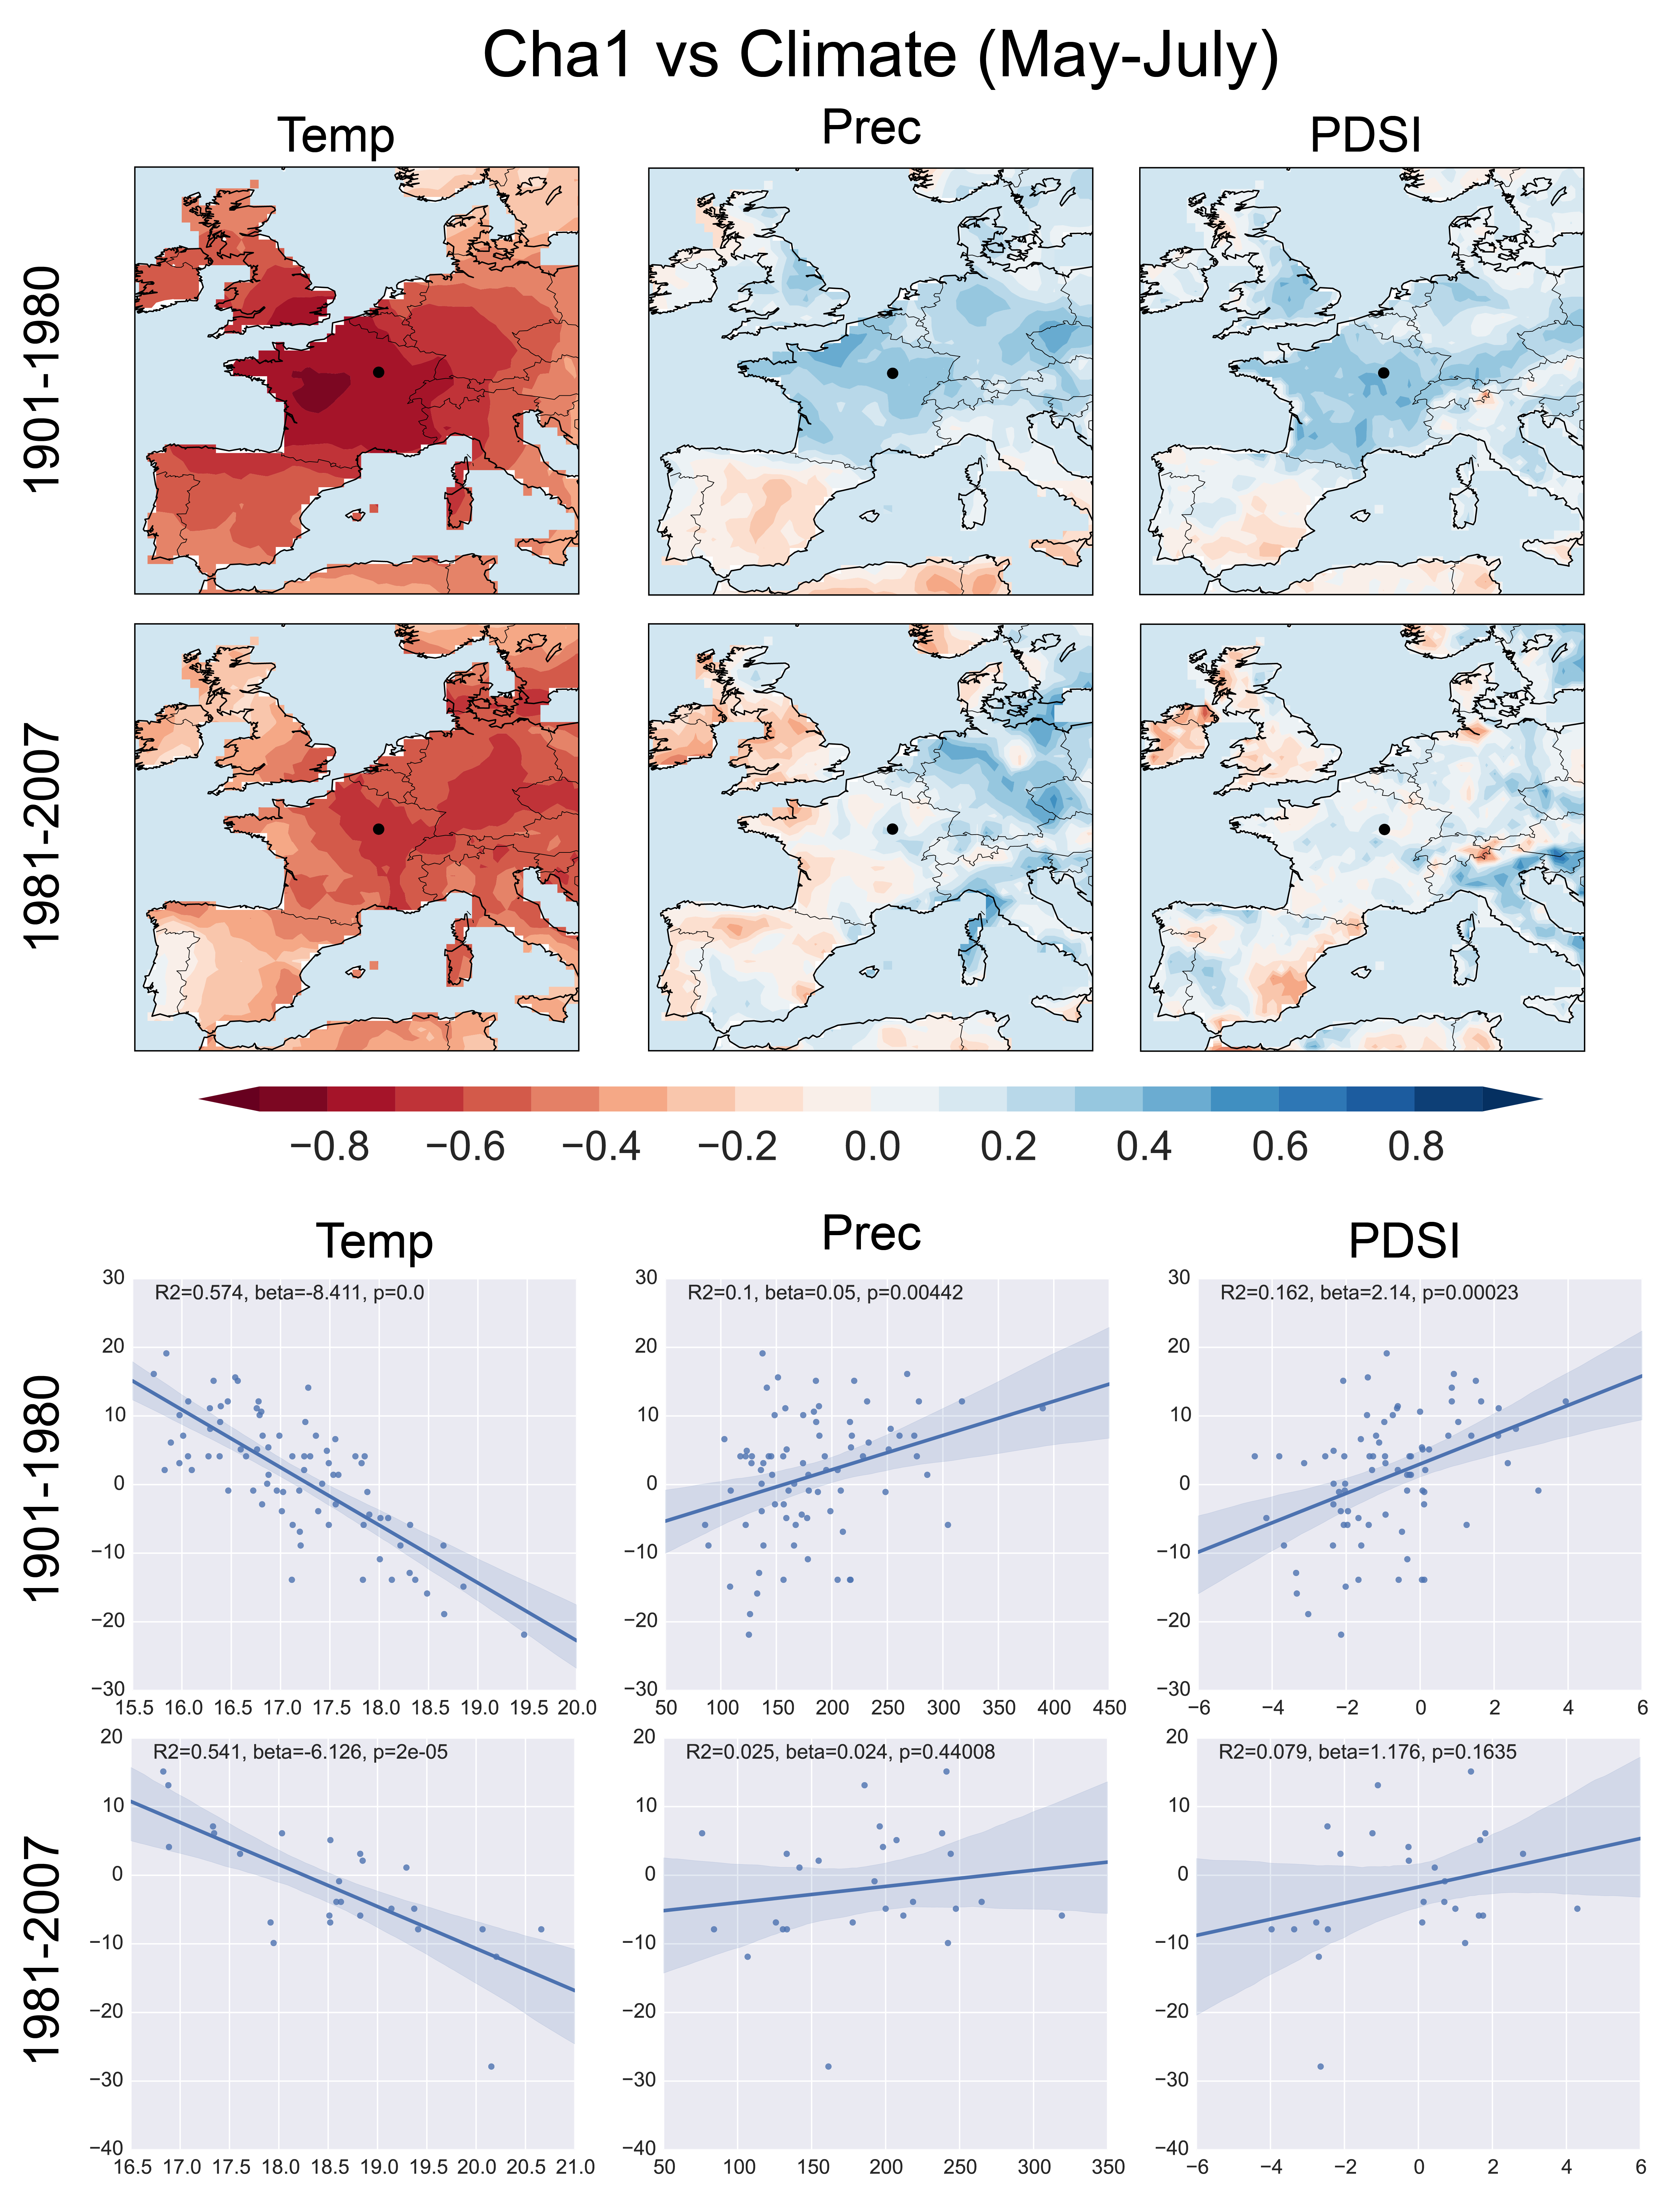
\includegraphics[width=.9\columnwidth,scale=2]{SUPP_fig_07_Cha1_MJJ_climate.png}
\caption{Same as Figure 4, but for Cha1.}
\end{figure}

\begin{figure}
\center
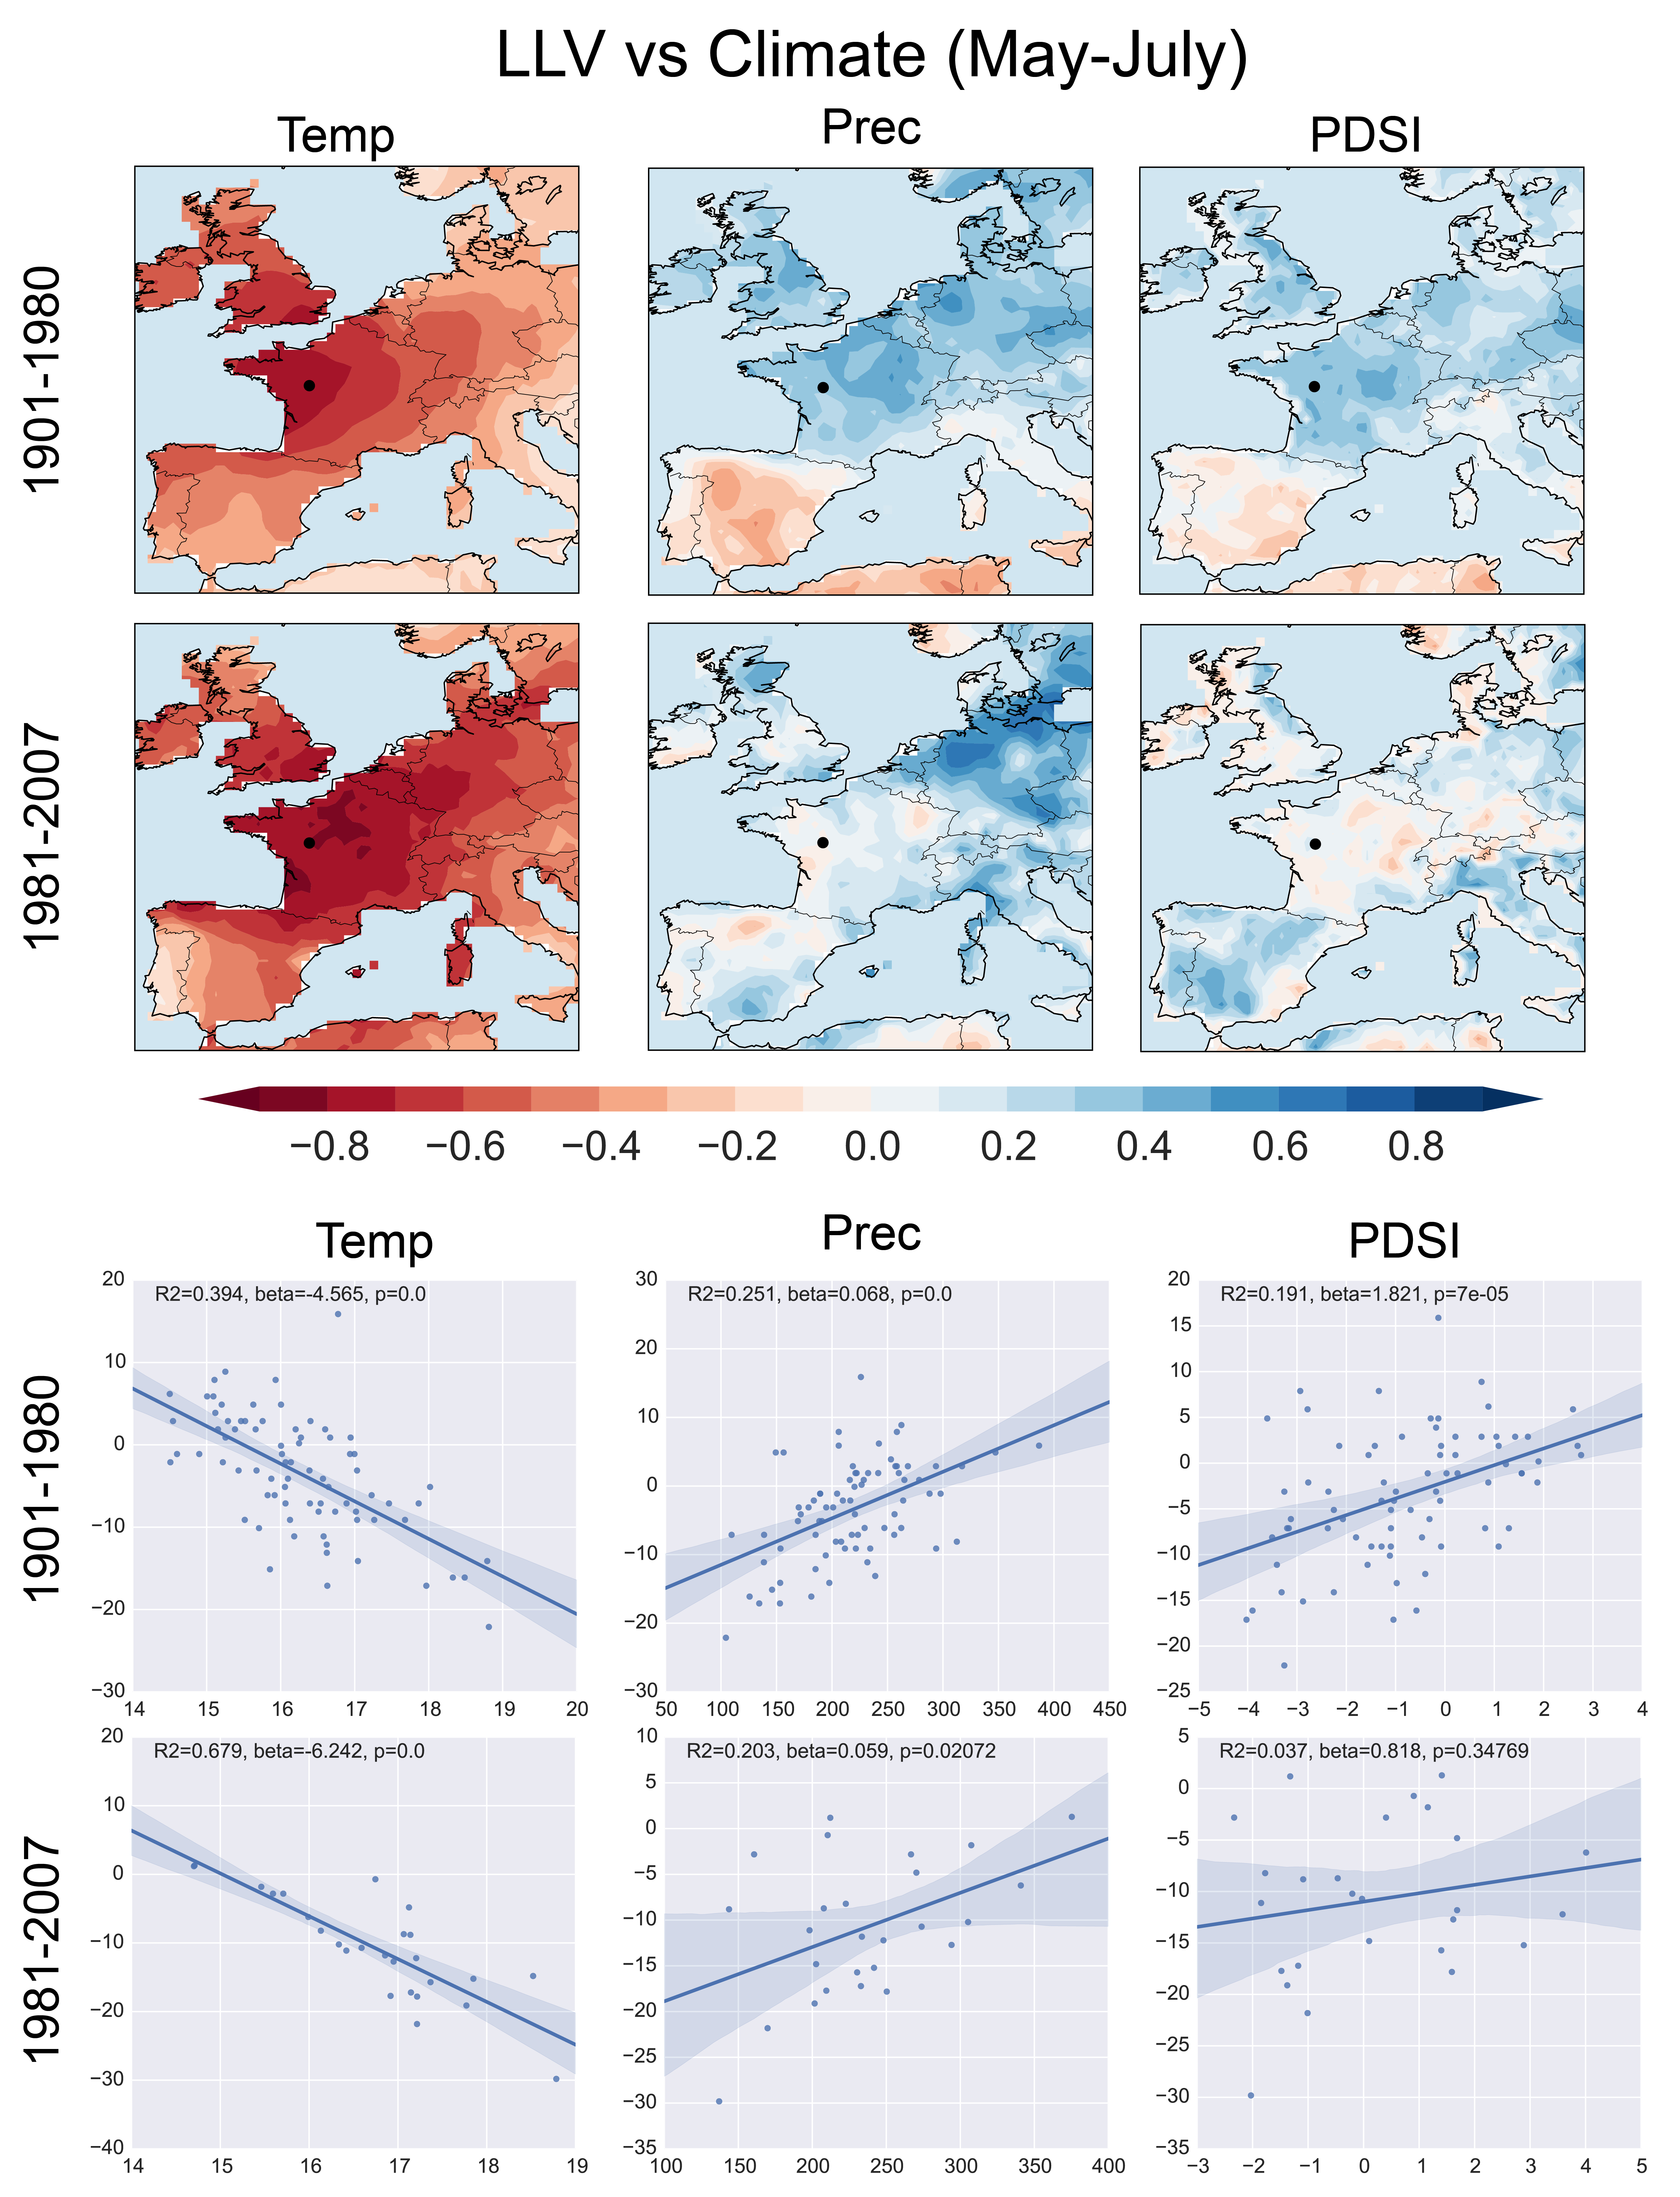
\includegraphics[width=.9\columnwidth,scale=2]{SUPP_fig_08_LLV_MJJ_climate.png}
\caption{Same as Figure 4, but for LLV.}
\end{figure}

\begin{figure}
\center
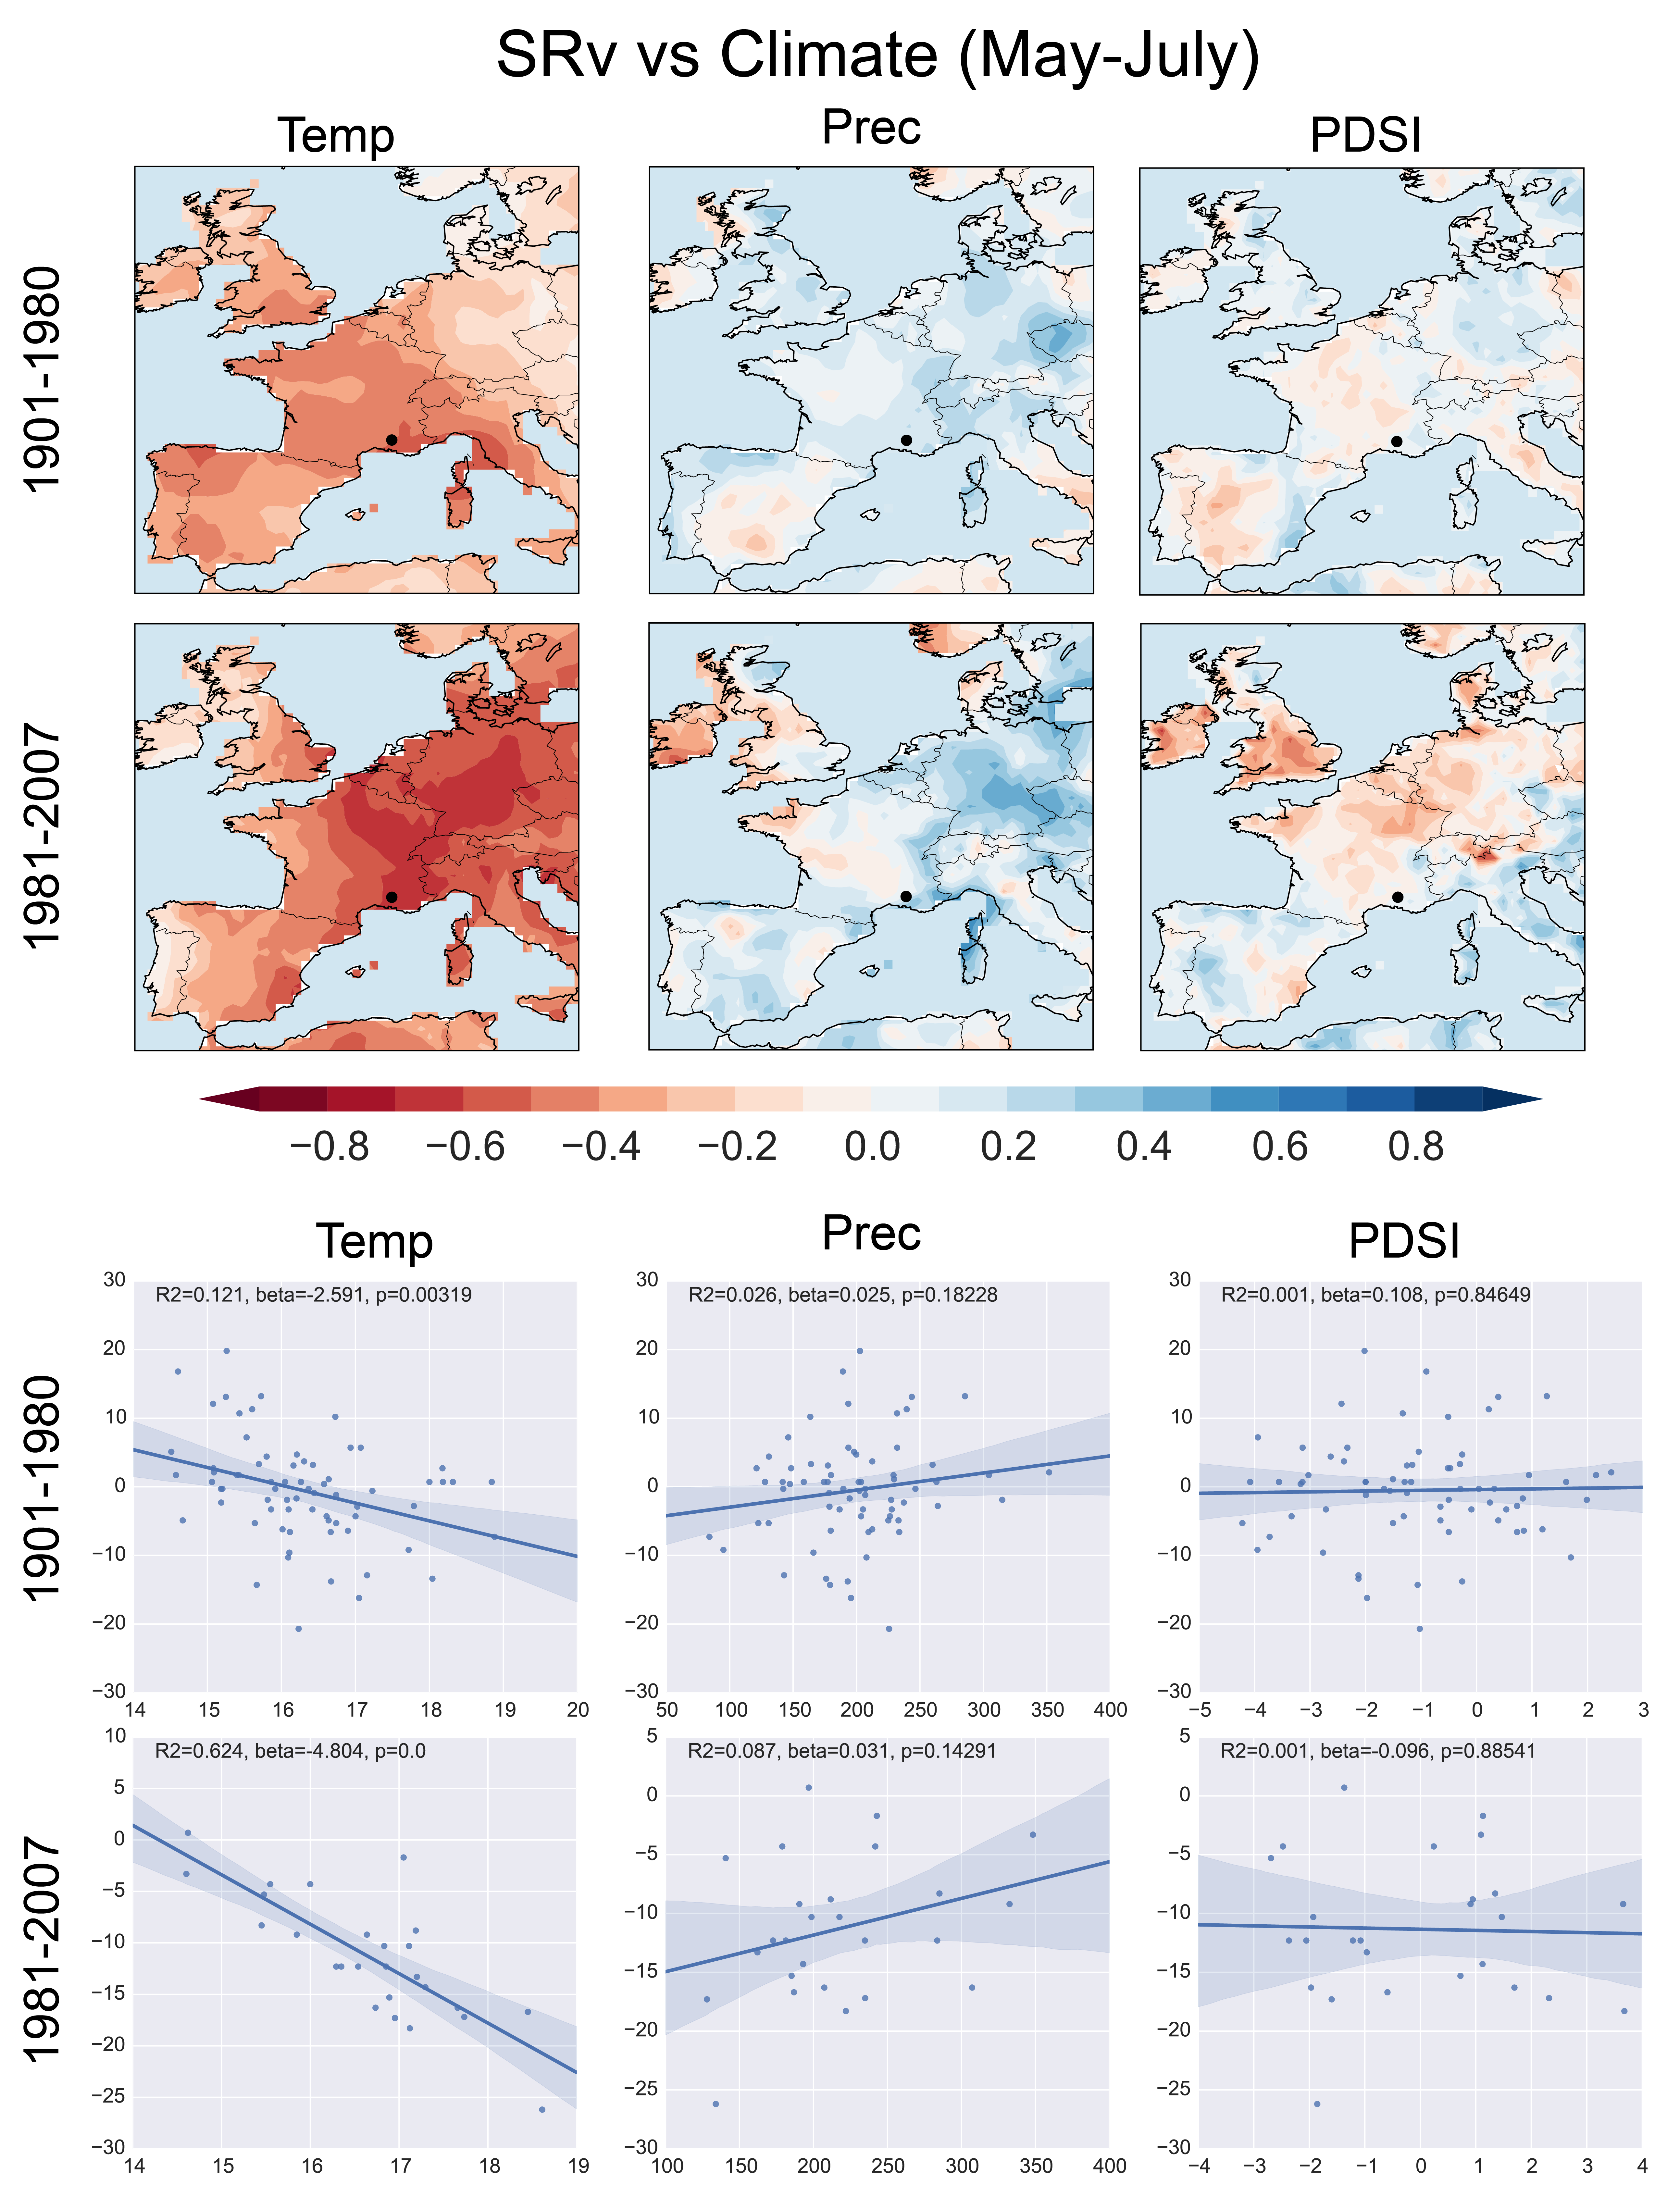
\includegraphics[width=.9\columnwidth,scale=2]{SUPP_fig_09_SRv_MJJ_climate.png}
\caption{Same as Figure 4, but for SRv.}
\end{figure}

\begin{figure}
\center
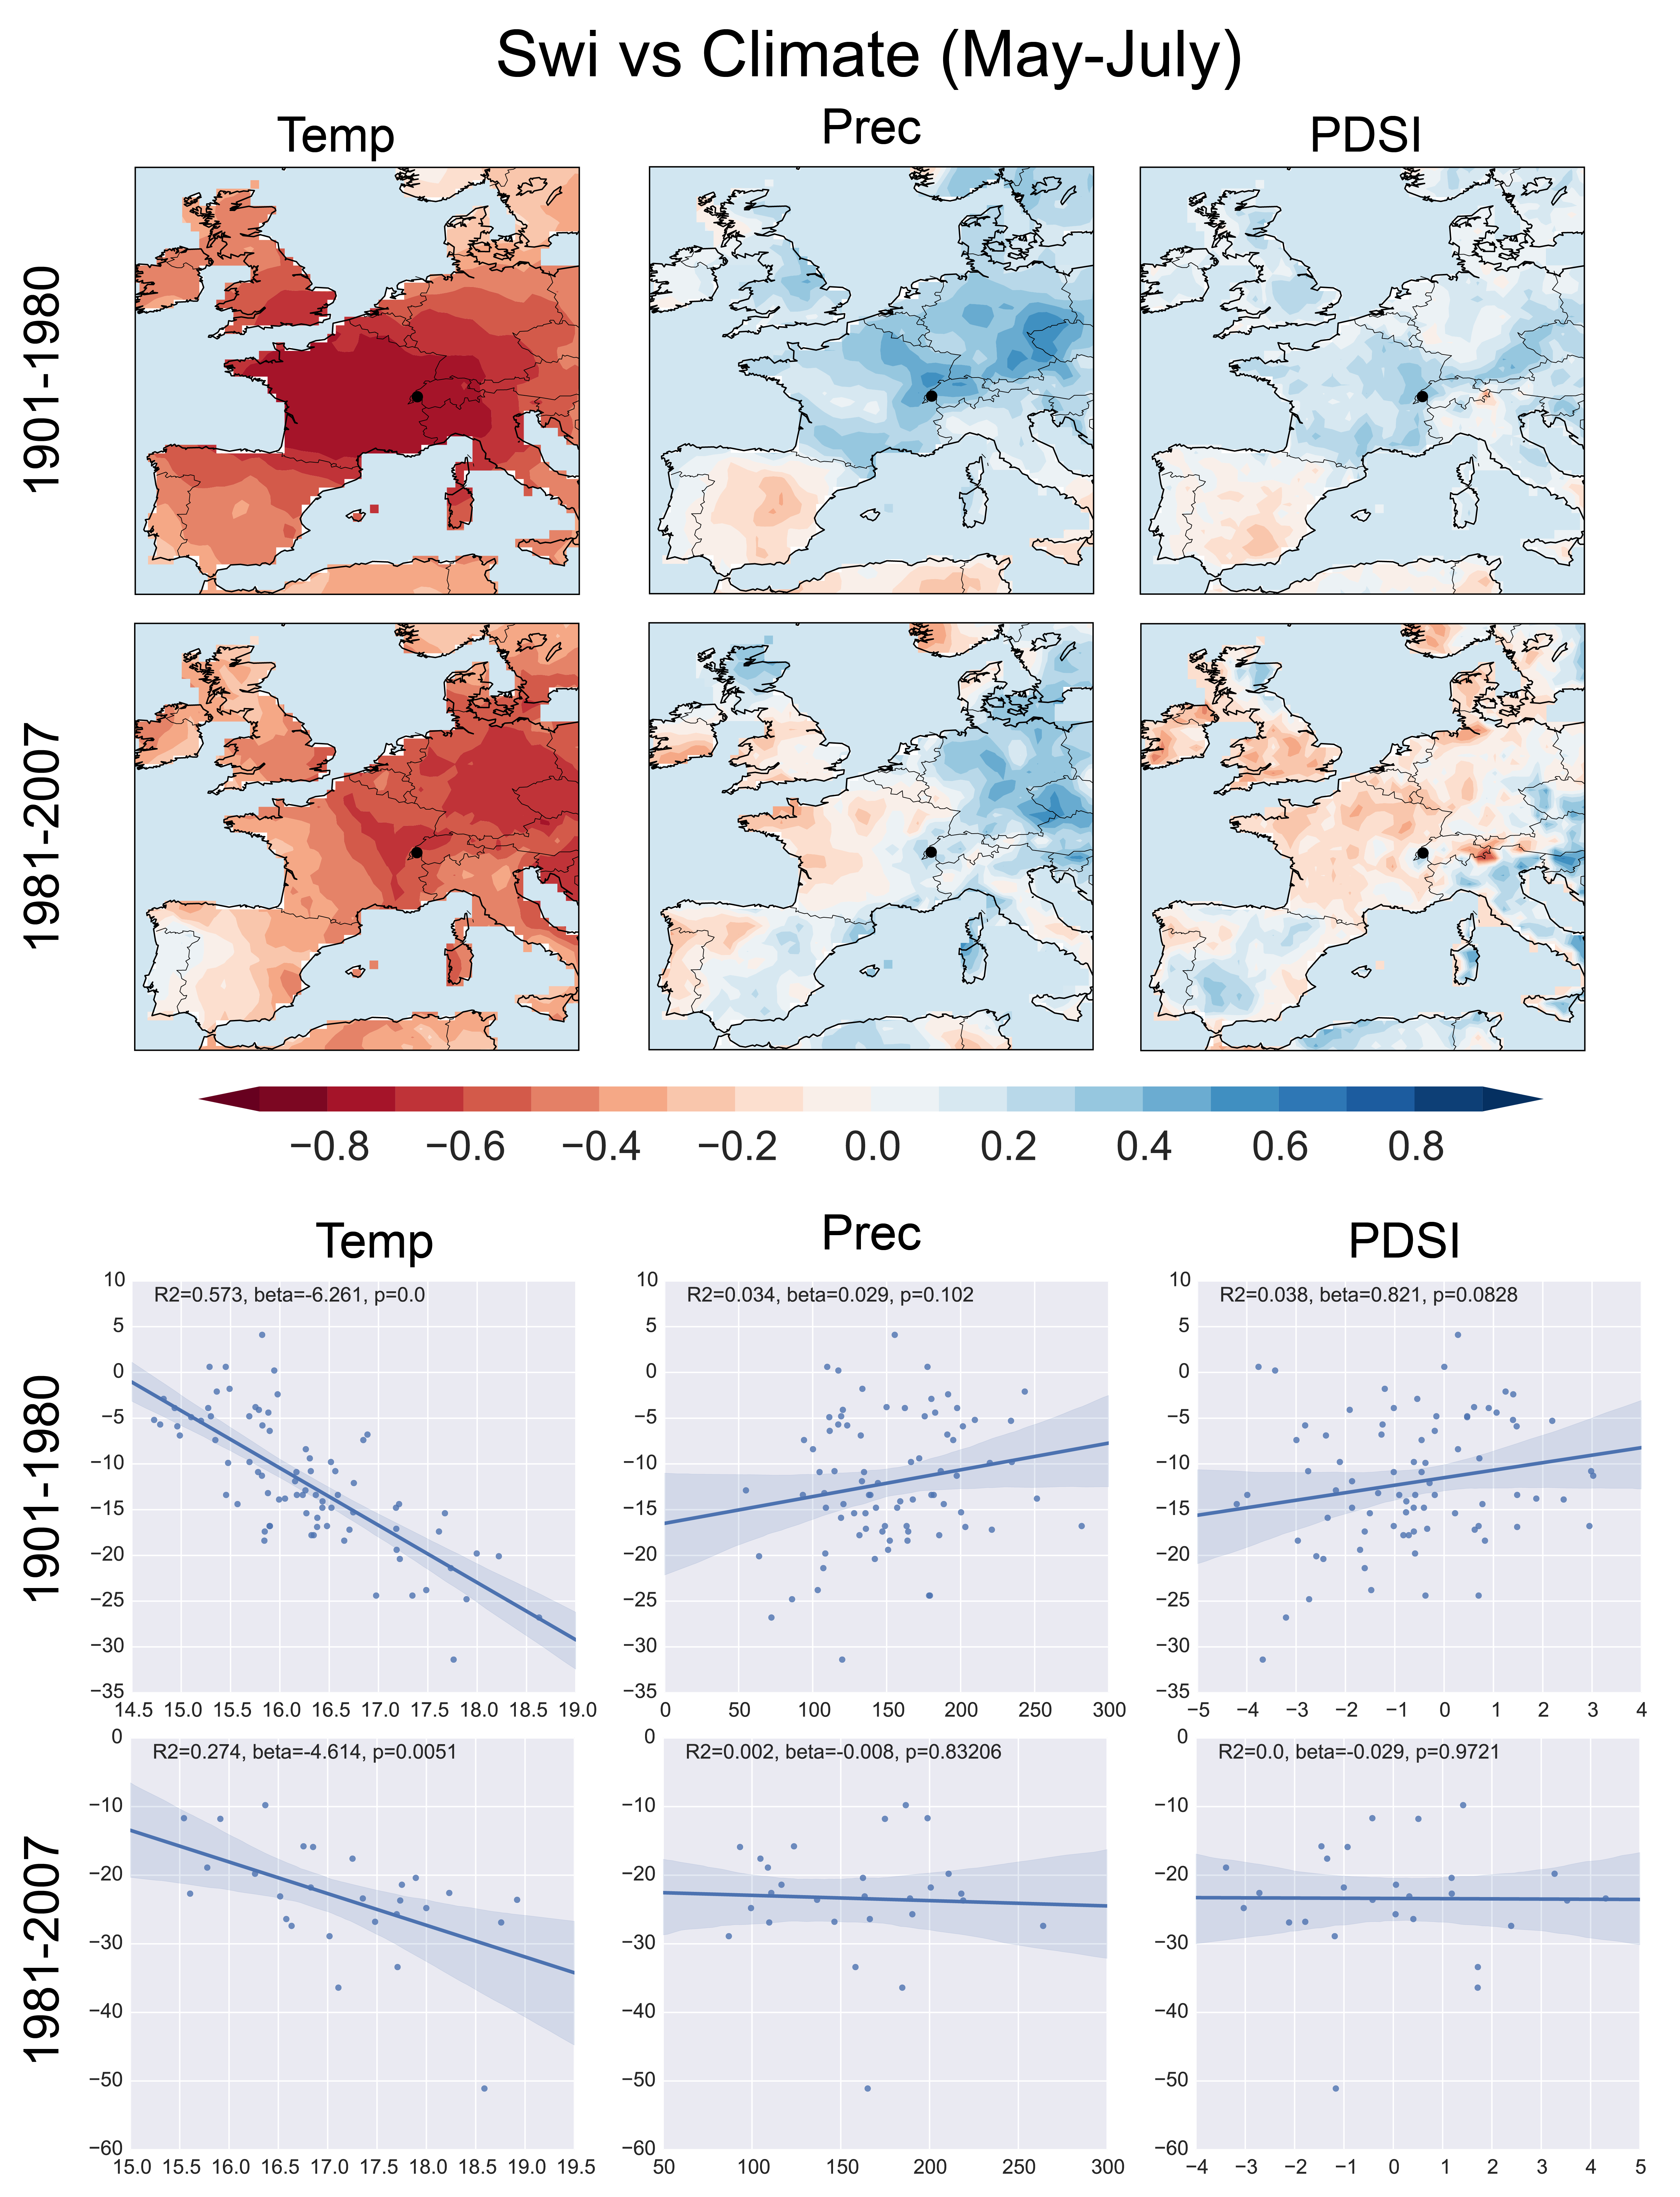
\includegraphics[width=.9\columnwidth,scale=2]{SUPP_fig_10_SWi_MJJ_climate.png}
\caption{Same as Figure 4, but for SWi.}
\end{figure}

\end{document}









